\documentclass[12pt,a4paper]{report}
\usepackage[utf8]{inputenc}
\usepackage[armenian,english]{babel}
\usepackage{graphicx}
\usepackage{geometry}
\usepackage{amsmath}
\usepackage{hyperref}
\usepackage{xurl}
\usepackage{caption}
\usepackage{float}
\usepackage{booktabs}
\usepackage{setspace}

\geometry{margin=1in}
\onehalfspacing

\title{Advanced Data-Driven Analysis of the Armenian Economy \\ \large Nowcasting Growth, Structural Shifts, and Macroeconomic Stability}
\author{Master's Thesis}
\date{2025}

\begin{document}

\maketitle
\tableofcontents

\chapter*{Abstract}
This thesis examines the short-run performance of the Armenian economy through a high-frequency analytical framework that combines official statistics, administrative indicators, and a custom GDP nowcasting dashboard (accessible at \url{https://haykozaq-gdp-nowcasting-dashboard-ogckd1.streamlit.app/}). The core research question is whether Armenia's post-2022 growth model has shifted from temporary shock-driven expansion toward a more durable structure based on construction, services, and information technology, while preserving macroeconomic stability. The empirical strategy uses monthly and quarterly indicators for commodity prices, tourism, remittances, economic activity, sectoral output, labor market dynamics, inflation, fiscal developments, and banking exposure. Rather than treating the dashboard as a collection of charts, the study organizes these indicators into an integrated interpretation of growth drivers, transmission channels, and vulnerabilities. The results suggest that Armenia entered 2025 with resilient momentum, but the composition of growth became increasingly uneven: construction and urban real estate remained dominant, ICT retained strategic importance, labor market conditions tightened, and fiscal as well as financial concentration risks became more visible. The thesis concludes that Armenia's near-term outlook remains favorable only if rapid sectoral expansion is matched by stronger productivity growth, disciplined macroeconomic management, and a gradual rebalancing away from excessive dependence on construction-led demand.

\chapter{Introduction}
\section{Research Motivation}
Armenia is a small open economy exposed to external shocks, migration flows, commodity price cycles, and regional geopolitical instability. In such an environment, annual national accounts alone are not sufficient for timely economic interpretation. Policymakers, firms, and researchers need high-frequency signals that reveal whether growth is broad-based, whether inflationary or financial pressures are building, and whether labor and external-sector dynamics are improving or weakening.

The Armenian case is especially important because the rapid expansion observed after 2022 contained both temporary and structural elements. Temporary factors included migration-related inflows, remittance surges, and abrupt trade re-routing. Structural factors included the scaling of the ICT sector, shifts in tourism composition, and a prolonged construction boom. The central analytical challenge is to distinguish normalization from deterioration and structural change from cyclical noise.

\section{Research Question and Objectives}
This thesis addresses the following main research question:

\begin{quote}
What are the main short-run drivers of Armenian economic growth in 2024--2025, and to what extent can high-frequency indicators nowcast changes in growth, labor-market conditions, and macroeconomic stability?
\end{quote}

The study has four objectives:
\begin{enumerate}
    \item to build an integrated high-frequency view of the Armenian economy using the dashboard indicators;
    \item to identify the sectors and channels that contributed most to growth normalization in 2024--2025;
    \item to assess whether observed growth was balanced across the real, external, labor, fiscal, and financial sectors;
    \item to evaluate the main macroeconomic risks associated with Armenia's current growth model.
\end{enumerate}

\section{Contribution}
The contribution of the thesis is practical as well as analytical. Practically, it consolidates a fragmented set of official and market indicators into a single dashboard-oriented framework. Analytically, it moves beyond descriptive chart presentation by linking the indicators to an explicit macroeconomic narrative: external shocks affect Armenia through commodity prices, trade, remittances, and exchange rates; these channels influence domestic production, employment, wages, and prices; and the resulting growth pattern shapes fiscal and banking-system exposure.

\section{Structure of the Thesis}
The remainder of the thesis proceeds as follows. Chapter 2 reviews the conceptual literature on nowcasting and growth analysis in small open economies. Chapter 3 presents the data and methodology behind the dashboard and nowcasting logic. Chapters 4 through 7 analyze Armenia's external sector, real activity, labor market, and macro-financial stability. Chapter 8 integrates the findings into a unified interpretation of Armenia's growth model. Chapter 9 discusses limitations. Chapter 10 concludes.

\chapter{Literature Review and Analytical Framework}
\section{Nowcasting in Small Open Economies}
Nowcasting refers to the estimation of current economic conditions before complete national accounts are released. In the literature, nowcasting methods typically rely on bridge equations, factor models, mixed-frequency regressions, or indicator-based composite systems. Their advantage is timeliness; their weakness is that high-frequency indicators may reflect noise, revisions, or temporary co-movement rather than stable economic relationships.

For a small open economy such as Armenia, nowcasting is particularly useful because major turning points can emerge first in trade, remittances, migration, commodity prices, exchange rates, and sector-specific monthly indicators. However, the same openness creates identification challenges. A strong tourism month, for example, may reflect seasonality rather than structural competitiveness; construction booms may raise GDP in the short run while creating medium-term financial vulnerabilities; and large migration flows may temporarily lift consumption, labor supply, and housing demand at the same time.

\section{Analytical Approach of This Thesis}
This thesis uses a dashboard-based empirical approach rather than a purely econometric one. The argument is not that a single model can fully explain Armenia's growth path, but that a disciplined combination of high-frequency indicators can reveal the changing composition of growth. The framework follows three principles:
\begin{enumerate}
    \item indicators are grouped by transmission channel rather than by data source alone;
    \item interpretation emphasizes consistency across multiple figures rather than isolated chart movements;
    \item strong causal claims are avoided unless supported by more than one indicator.
\end{enumerate}

Accordingly, the thesis evaluates Armenia's economy through five linked channels: external conditions, real-sector activity, labor and demographics, prices and policy, and financial concentration. This structure is more appropriate for the Armenian case than a purely sectoral description because the same shock may propagate through several channels simultaneously.

\chapter{Data and Methodology}
\section{Data Sources}
The deployed version of the dashboard is available at \url{https://haykozaq-gdp-nowcasting-dashboard-ogckd1.streamlit.app/}. The dashboard combines monthly and quarterly indicators from the main Armenian and international statistical sources. The core domestic sources are the Statistical Committee of the Republic of Armenia (Armstat), the Central Bank of Armenia (CBA), and the Ministry of Finance. International context variables are taken from publicly available commodity and macroeconomic datasets used in IMF, World Bank, and ADB assessments. The figures included in this thesis are based on processed datasets stored in the project workspace and transformed into publication-ready visuals.\cite{armstatbank,cbaMPR2025Q1,minfinBudget,imfCR24348,wbMEU2025,adbADO2024}

The indicator set covers:
\begin{itemize}
    \item commodity prices: oil, copper, gold, and international food prices;
    \item external demand and inflows: tourism, remittances, trade, and exchange rates;
    \item real activity: economic activity index, industrial output, agriculture, and construction;
    \item labor market: employment, unemployment, labor resources, migration, and wages;
    \item macro-financial conditions: CPI, budget revenue and expenditure, utilities, and credit composition.
\end{itemize}

\section{Time Coverage and Interpretation Rules}
The dashboard uses the latest monthly and quarterly observations available at the time of compilation. Because some series are reported with lags and others cover only part of the year, the analysis distinguishes three types of evidence:
\begin{enumerate}
    \item \textbf{realized observations}, where complete official data are available;
    \item \textbf{partial-year assessments}, where trends are inferred from year-to-date information;
    \item \textbf{nowcast-based interpretation}, where current conditions are approximated using high-frequency indicators before full GDP release.
\end{enumerate}

This distinction is essential. A chart labeled for 2025 should not automatically be interpreted as a full-year outcome. In this thesis, figure-based analysis refers to the observation window represented in the underlying data, not to a guaranteed year-end realization.

\section{Nowcasting Logic}
The nowcasting framework is indicator-based. It does not claim to be a full structural macroeconomic model. Instead, it tracks the current state of the economy by combining signals from sectors that historically co-move with Armenian GDP and the Economic Activity Index (EAI). The logic of the framework is as follows:
\begin{enumerate}
    \item monthly sector indicators are normalized to allow comparison across different units;
    \item indicators are grouped into macro blocks such as external demand, domestic activity, and labor conditions;
    \item sector contribution charts are used to identify whether growth is broad-based or concentrated;
    \item the nowcasted GDP path is interpreted jointly with EAI, construction, industry, tourism, and labor indicators.
\end{enumerate}

\section{Methodological Limitations}
Several limitations should be noted at the outset. First, Armenian macroeconomic data can be revised, especially when annual totals replace monthly estimates. Second, some indicators are better interpreted as leading signals than as direct measures of output. Third, correlation does not prove causation: a sector may expand at the same time as GDP without being the dominant reason for overall growth. Fourth, migration and geopolitical shocks may create structural breaks that weaken the predictive power of historical patterns. These limitations do not invalidate the dashboard, but they require cautious interpretation.\cite{imfCR24348,wbPulse2025}

\chapter{External Sector and Global Drivers}
\section{Commodity Markets, Terms of Trade, and Export Sensitivity}
Armenia's external position remains sensitive to commodity prices, especially through mining exports and imported energy costs. The commodity figures therefore serve as a first filter for understanding the broader macroeconomic environment.

\begin{figure}[H]
    \centering
    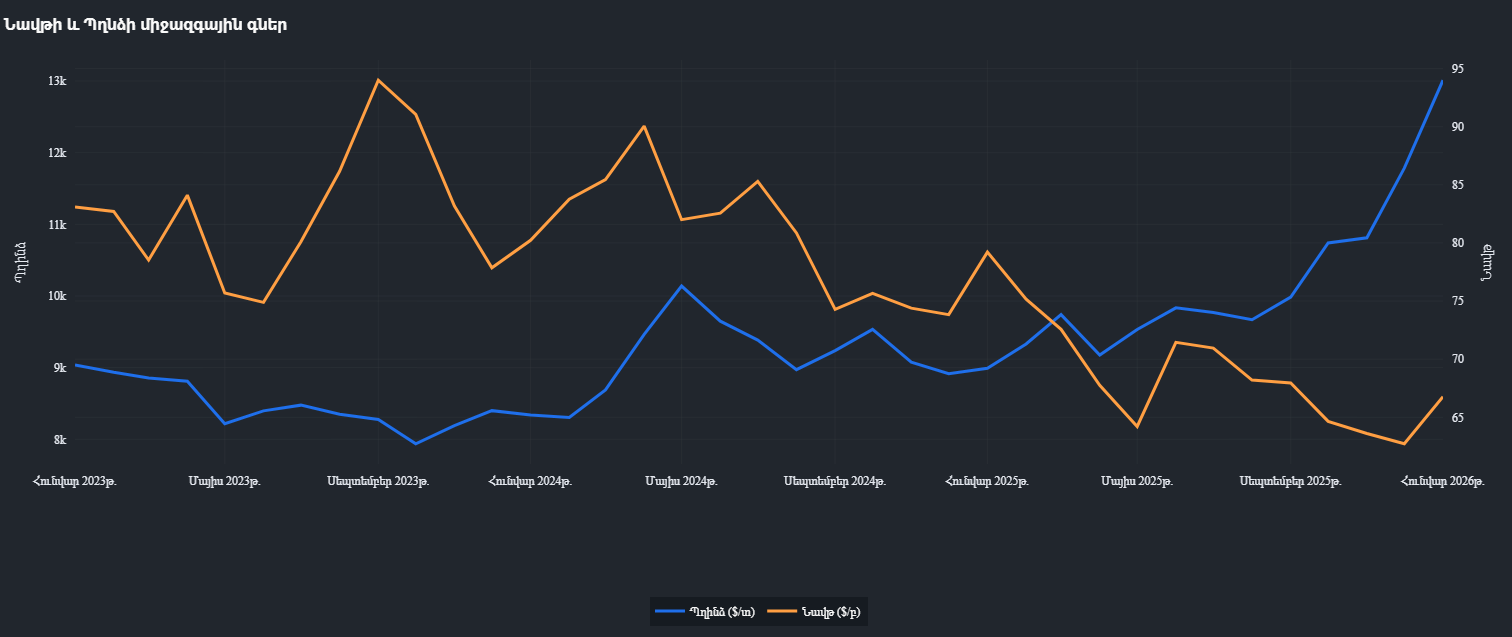
\includegraphics[width=0.8\textwidth]{figures/00_commodities_oil_copper.png}
    \caption{Global Market Trends: Oil and Copper Prices (2025)}
    \label{fig:oil_copper}
\end{figure}

\begin{figure}[H]
    \centering
    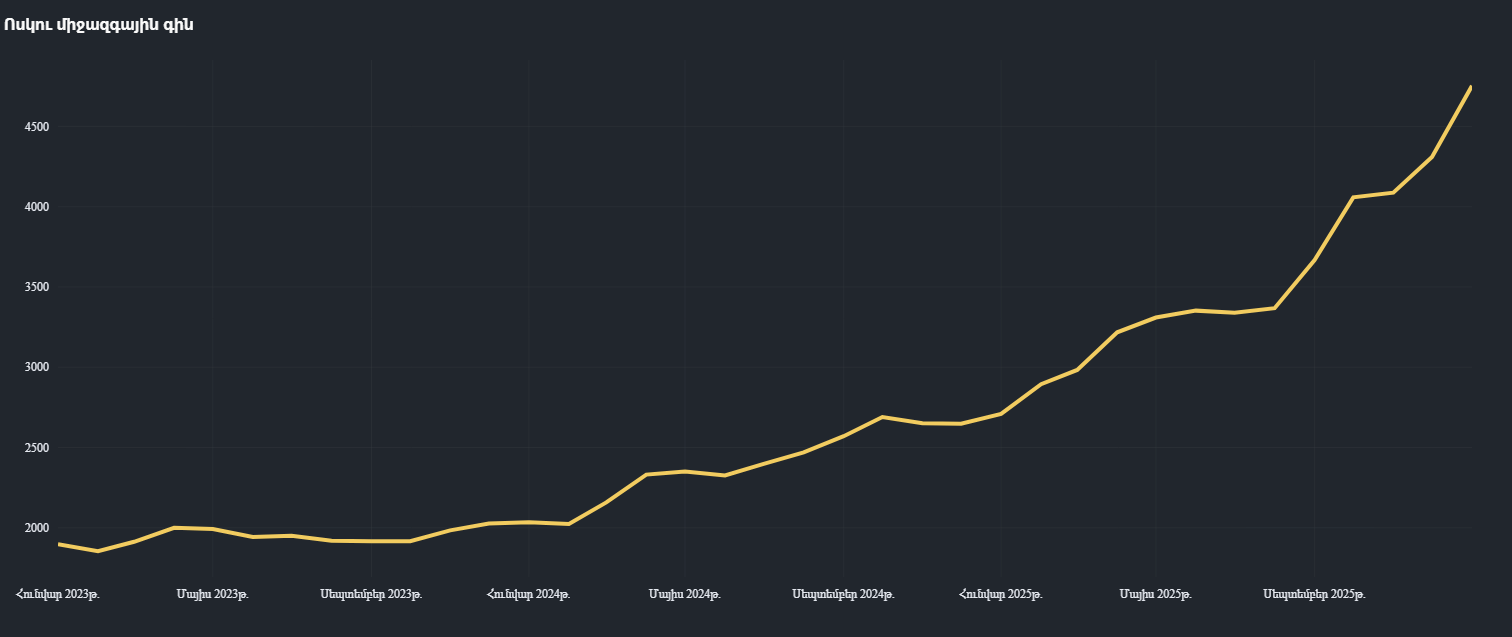
\includegraphics[width=0.8\textwidth]{figures/01_commodities_gold.png}
    \caption{Gold Price Volatility and its Impact on Armenian Export Portfolios}
    \label{fig:gold_prices}
\end{figure}

\begin{figure}[H]
    \centering
    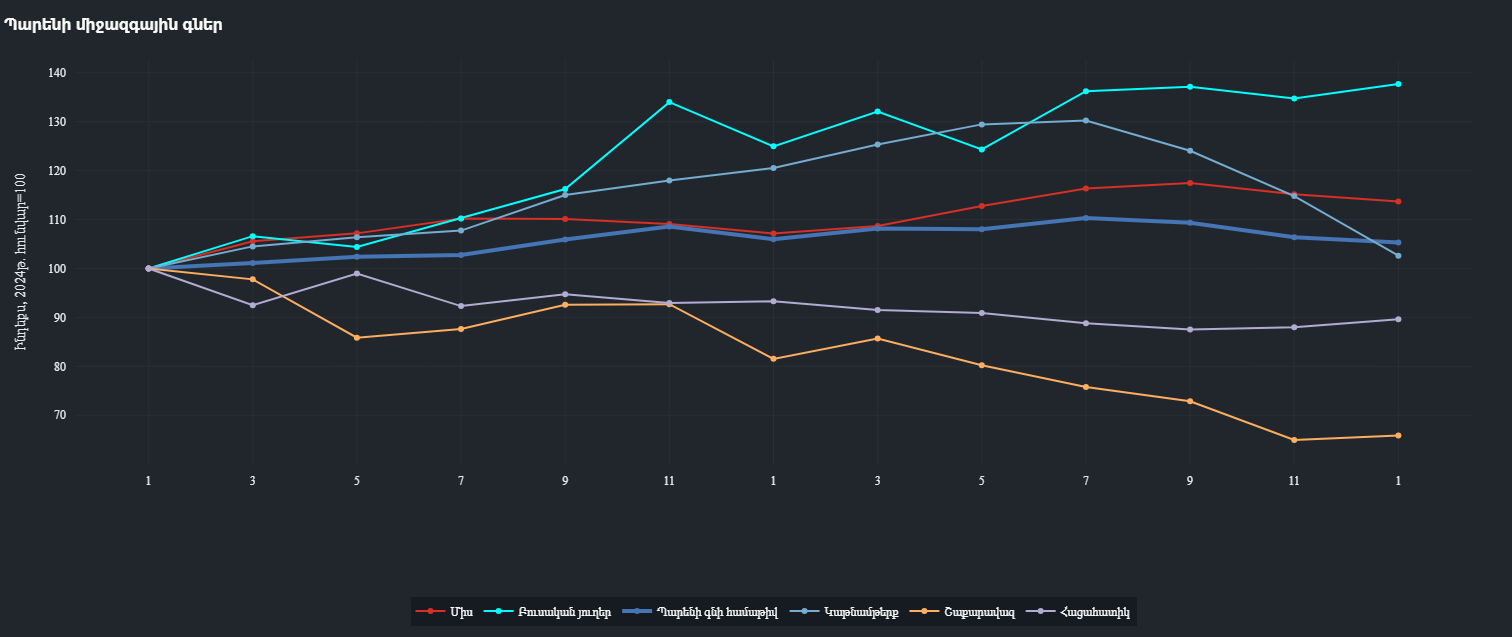
\includegraphics[width=0.8\textwidth]{figures/02_commodities_food_intl.png}
    \caption{International Food Price Index Trends}
    \label{fig:food_prices}
\end{figure}

Figures \ref{fig:oil_copper}--\ref{fig:food_prices} indicate why Armenia's growth outlook cannot be interpreted through domestic indicators alone. Higher gold prices support export earnings and can partially cushion weaker mining volumes, but this effect is not equivalent to a broad improvement in industrial competitiveness. Copper dynamics matter not only for mining revenues but also for Armenia's exposure to external demand conditions. International food price moderation, by contrast, supports lower imported inflation and creates room for more stable domestic price expectations. The analytical implication is that Armenia may simultaneously benefit from favorable external price conditions while remaining structurally dependent on a narrow set of export-linked variables.\cite{wbMEU2024,imfCR24348}

\section{Tourism and the Recomposition of Service Exports}
\begin{figure}[H]
    \centering
    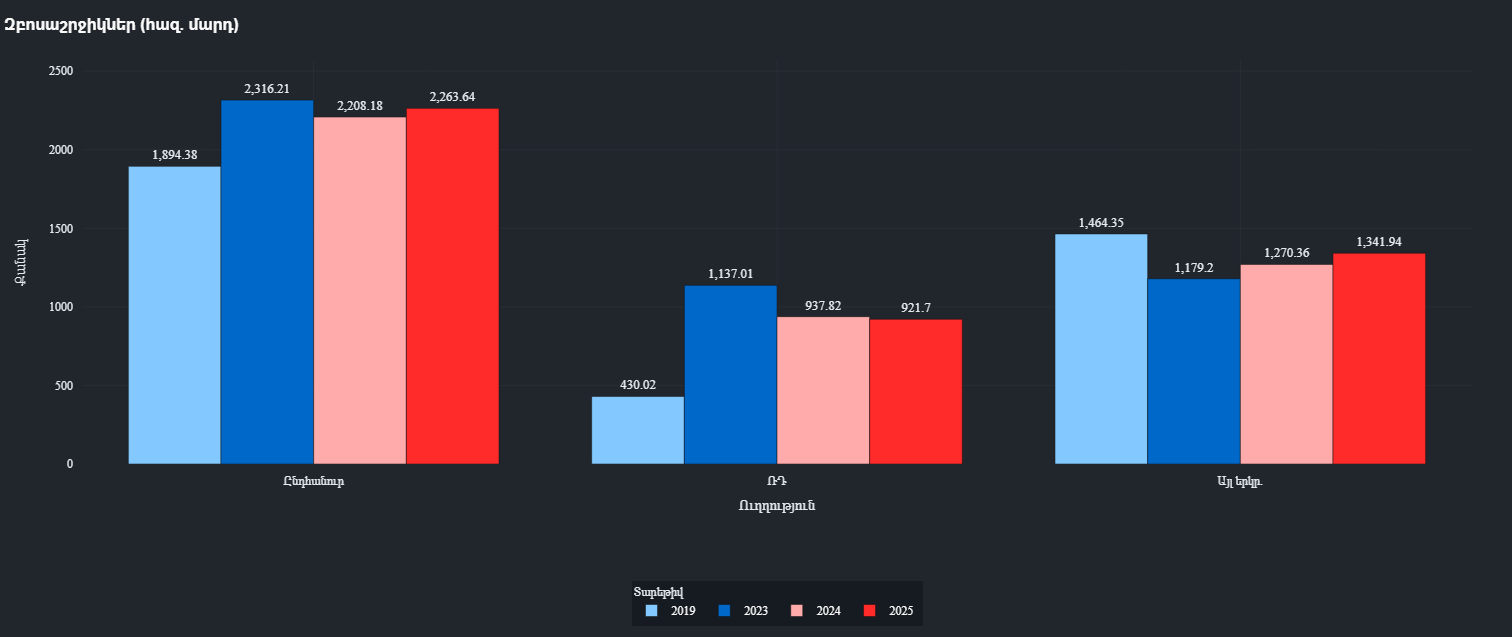
\includegraphics[width=0.8\textwidth]{figures/03_tourism_total.png}
    \caption{Total Tourist Arrivals: Monthly Comparison (2024 vs 2025)}
    \label{fig:tourism_total}
\end{figure}

\begin{figure}[H]
    \centering
    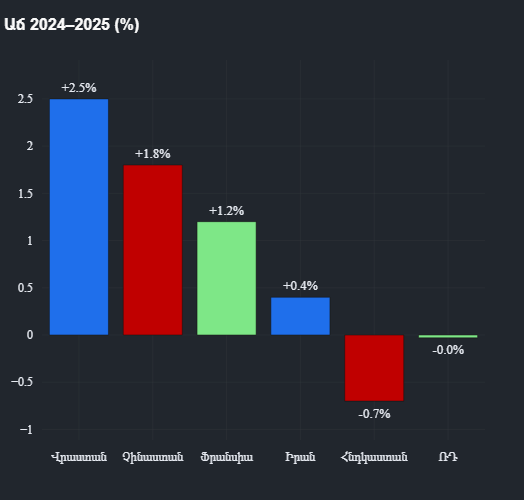
\includegraphics[width=0.8\textwidth]{figures/04_tourism_growth_dest.png}
    \caption{Tourism Growth by Visitor Destination and Origin}
    \label{fig:tourism_dest}
\end{figure}

Tourism is one of the clearest examples of why composition matters as much as scale. Figure \ref{fig:tourism_total} shows whether total flows remained resilient, while Figure \ref{fig:tourism_dest} provides the more important analytical signal: the origin structure of visitors. If growth is increasingly supported by a more diversified set of markets, then tourism earnings become less vulnerable to a single regional shock. That would represent a genuine structural improvement. If, however, the sector merely stabilizes after an earlier relocation-driven surge, then the interpretation should be normalization rather than sustained acceleration. The thesis therefore treats tourism as a channel of service-export resilience, but not as sufficient evidence of a permanently stronger growth regime on its own.\cite{armstatbank,wbTourism2025}

\section{Remittances, Exchange Rates, and External Liquidity}
\begin{figure}[H]
    \centering
    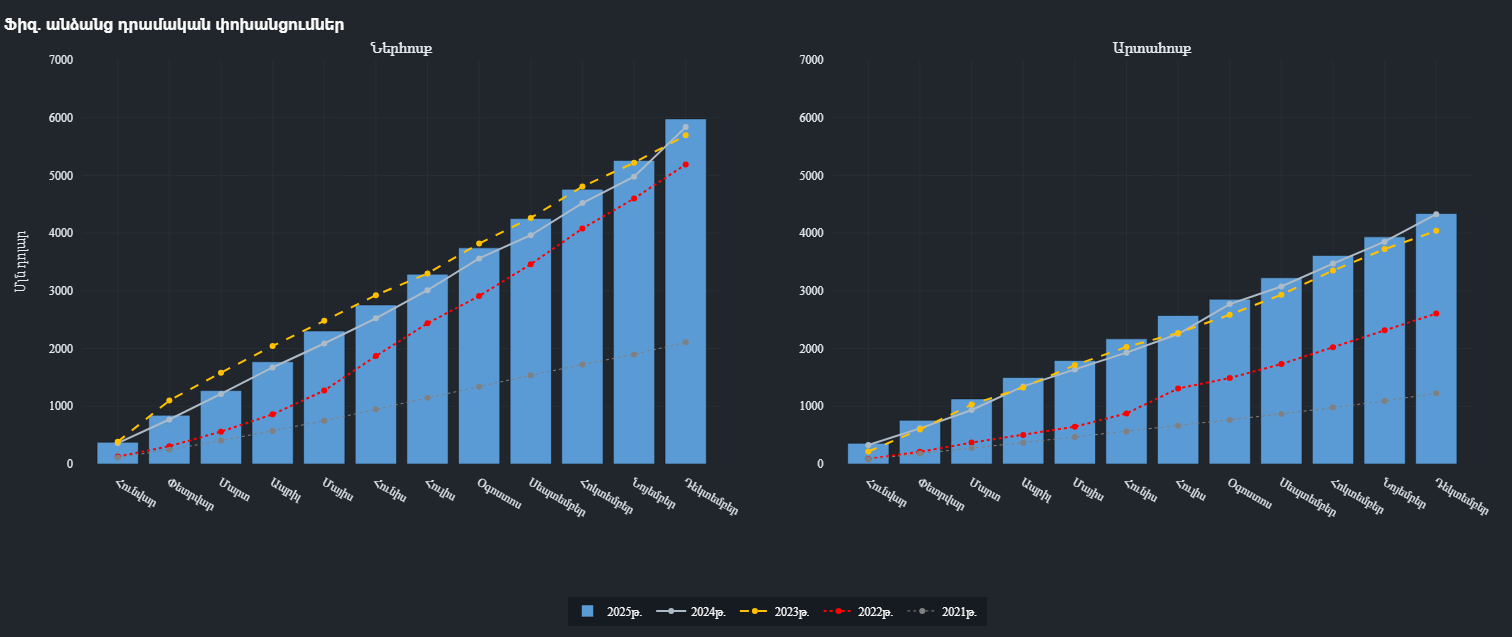
\includegraphics[width=0.8\textwidth]{figures/05_remittances_monthly_io.png}
    \caption{Remittance Inflows and Outflows (Monthly)}
    \label{fig:remittances_io}
\end{figure}

\begin{figure}[H]
    \centering
    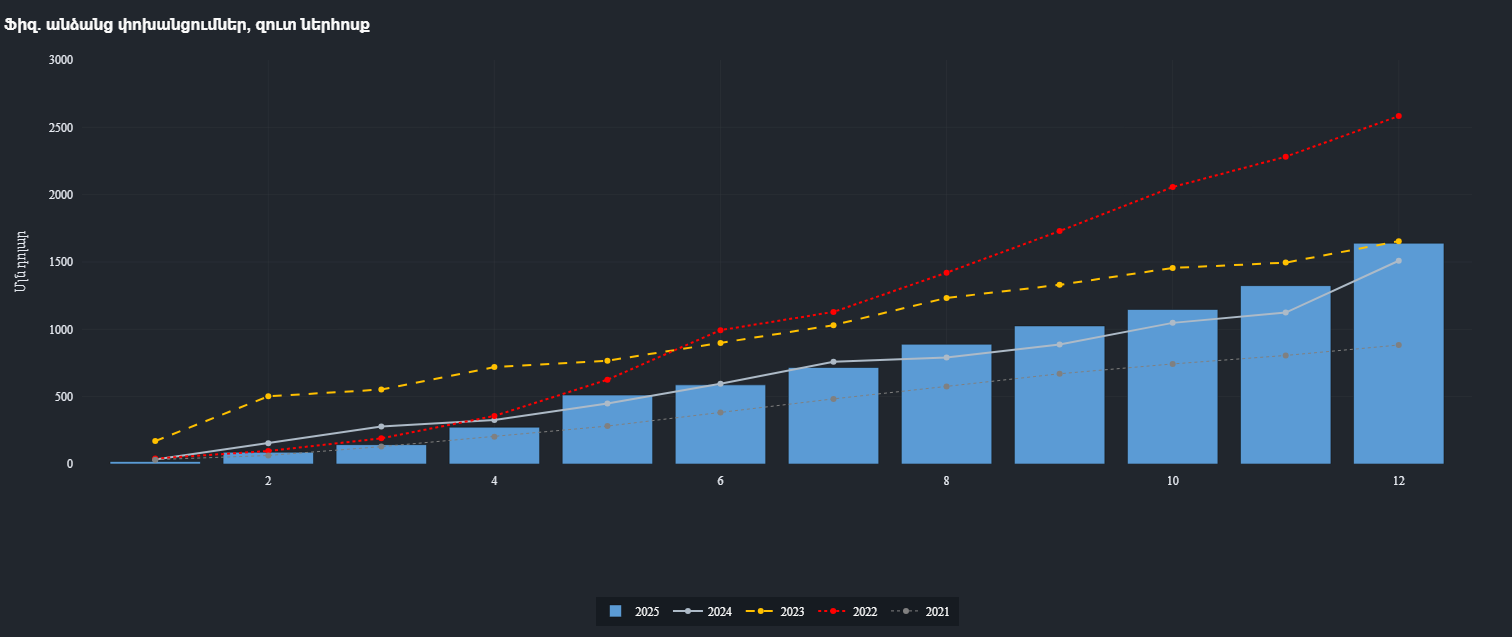
\includegraphics[width=0.8\textwidth]{figures/06_remittances_net.png}
    \caption{Net Remittance Impact on Disposable Income}
    \label{fig:remittances_net}
\end{figure}

\begin{figure}[H]
    \centering
    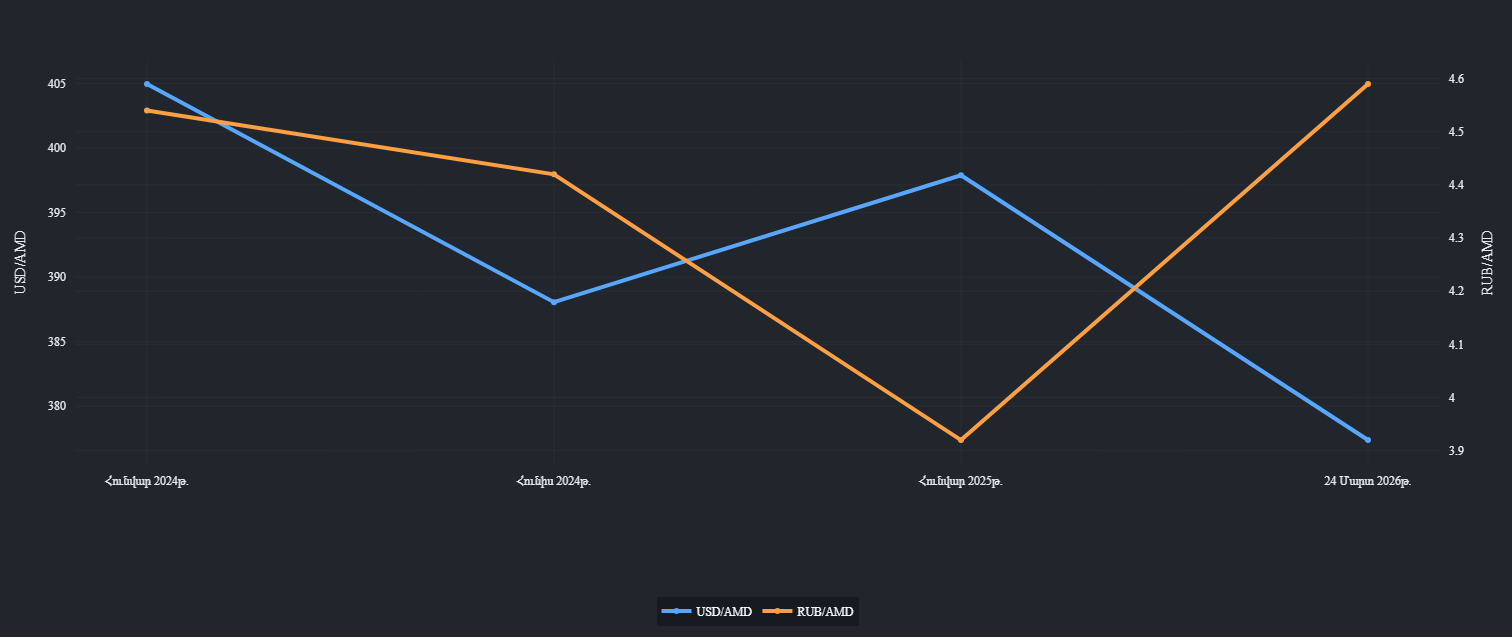
\includegraphics[width=0.8\textwidth]{figures/33_exchange_rates.png}
    \caption{Exchange Rate Dynamics: USD/AMD and RUB/AMD Trends}
    \label{fig:exchange_rates}
\end{figure}

Remittances and exchange-rate conditions are central to Armenian macroeconomic transmission. Figures \ref{fig:remittances_io} and \ref{fig:remittances_net} should be read not only as balance-of-payments indicators, but also as signals of household purchasing power, housing demand, and import capacity. Figure \ref{fig:exchange_rates} adds the monetary dimension: exchange-rate stability can help contain imported inflation, but excessive appreciation may weaken competitiveness in tradable sectors. The relevant analytical point is therefore not simply whether remittances stayed high, but whether Armenia's domestic demand and currency stability remained too dependent on external private inflows. That dependence is manageable in the short run, yet it becomes a vulnerability if inflows normalize faster than domestic productivity rises.\cite{cbaMPR2025Q1,imfCR24348,wbMEU2025}

\chapter{Real Sector Performance and Nowcasting Results}
\section{Growth Normalization and the Economic Activity Index}
\begin{figure}[H]
    \centering
    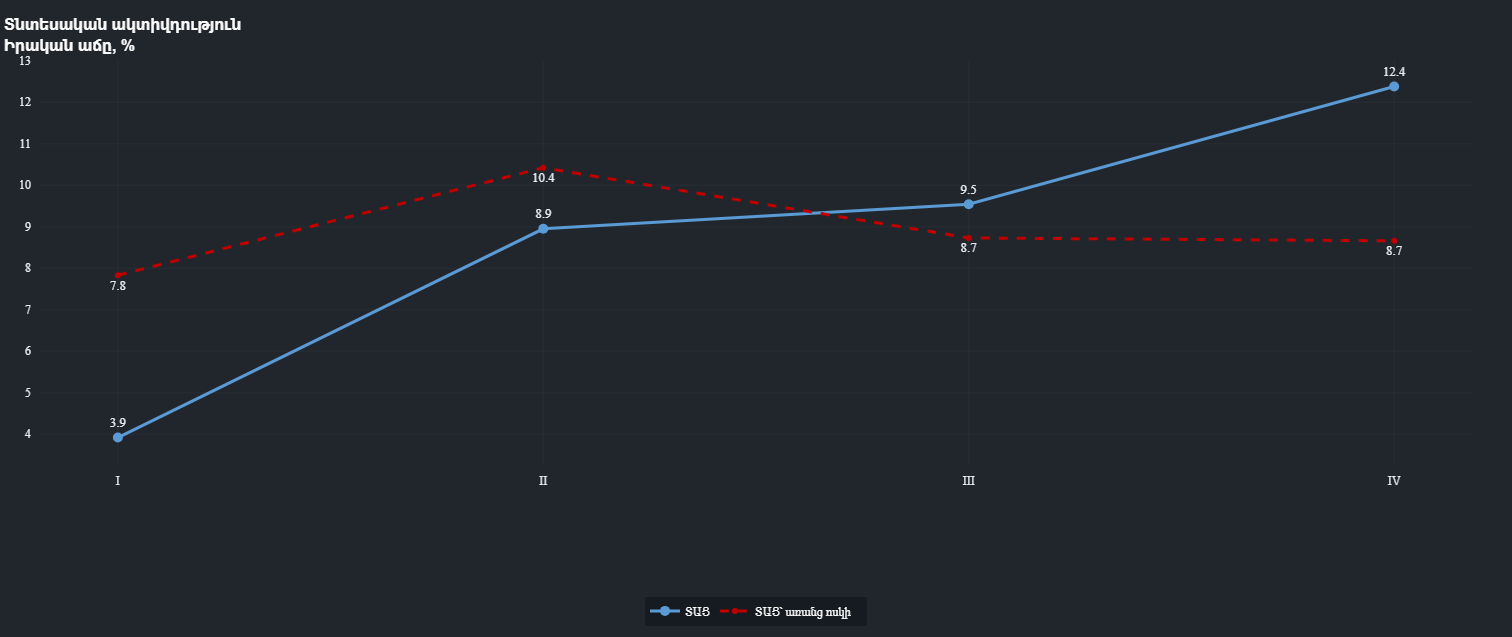
\includegraphics[width=0.8\textwidth]{figures/07_eai_quarterly_gold.png}
    \caption{Quarterly EAI Correlation with Gold Mining Activity}
    \label{fig:eai_gold}
\end{figure}

\begin{figure}[H]
    \centering
    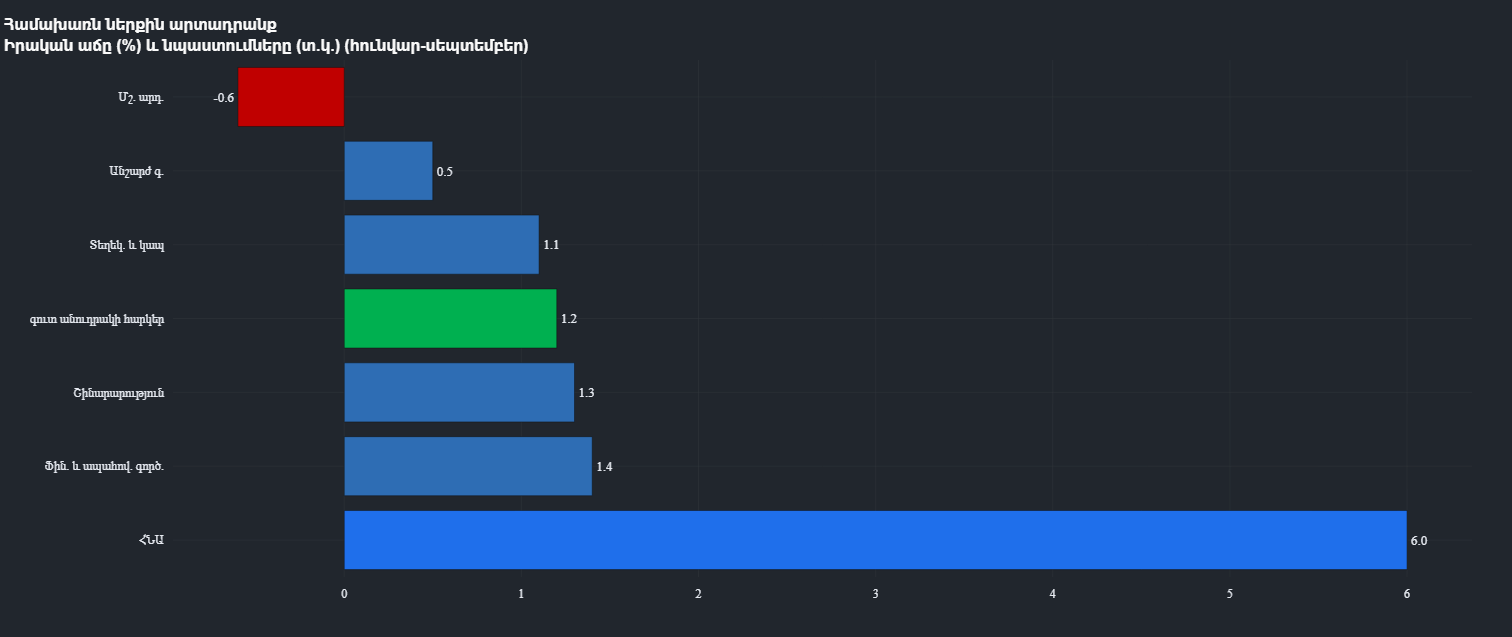
\includegraphics[width=0.8\textwidth]{figures/08_gdp_growth_2024.png}
    \caption{Annual GDP Growth Path: Monthly and Cumulative Targets (Nowcasted)}
    \label{fig:gdp_24}
\end{figure}

\begin{figure}[H]
    \centering
    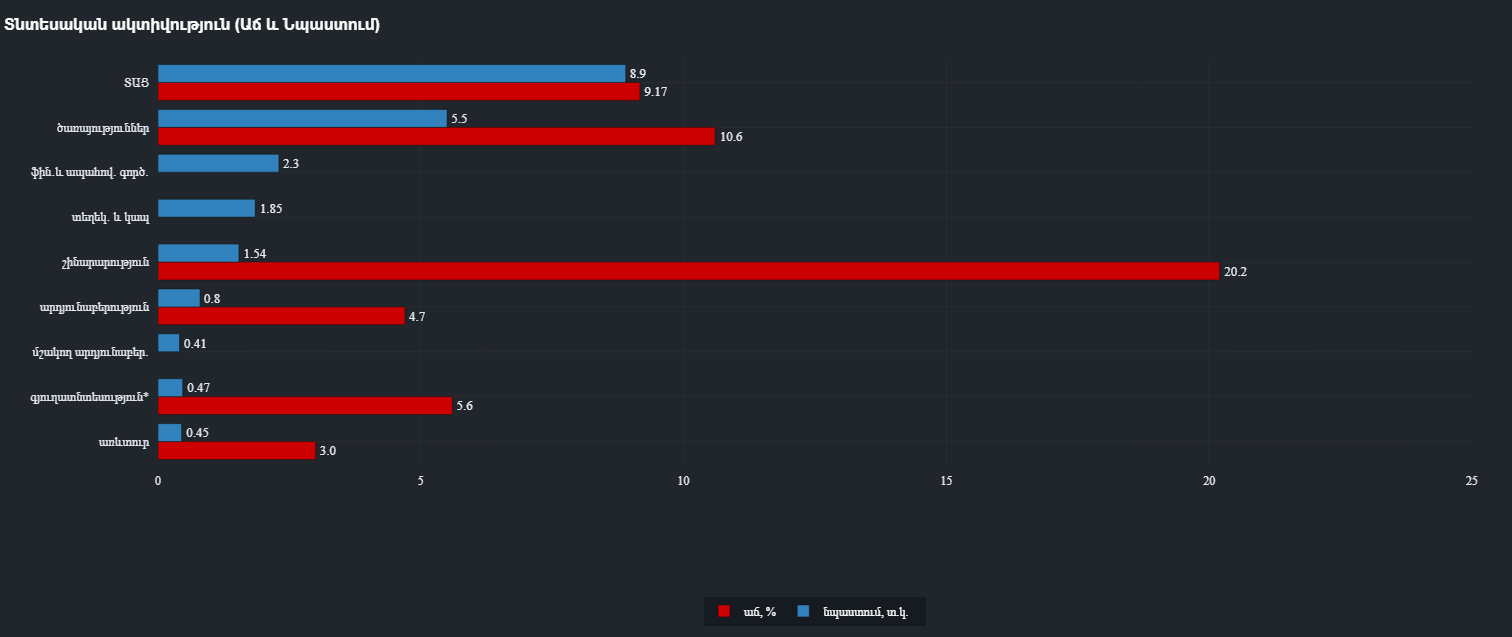
\includegraphics[width=0.8\textwidth]{figures/09_eai_sector_contributions.png}
    \caption{Sectoral Contributions to the Economic Activity Index}
    \label{fig:eai_sectors}
\end{figure}

The core output question of the thesis is not whether Armenia grew, but how it grew. Figure \ref{fig:gdp_24} suggests that the economy remained on a positive expansion path, but the more important evidence comes from Figures \ref{fig:eai_gold} and \ref{fig:eai_sectors}. These indicate whether aggregate growth was supported by diversified sectoral momentum or by a narrow set of high-performing activities. A thesis-grade interpretation must therefore focus on concentration. If the EAI is increasingly explained by services and construction, then headline growth may still look strong while medium-term balance deteriorates. The nowcasting contribution of the dashboard lies exactly here: it helps identify composition before full annual GDP accounts are published.\cite{armstatbank,wbPulse2025,adbADO2024}

\section{Industry and Manufacturing}
\begin{figure}[H]
    \centering
    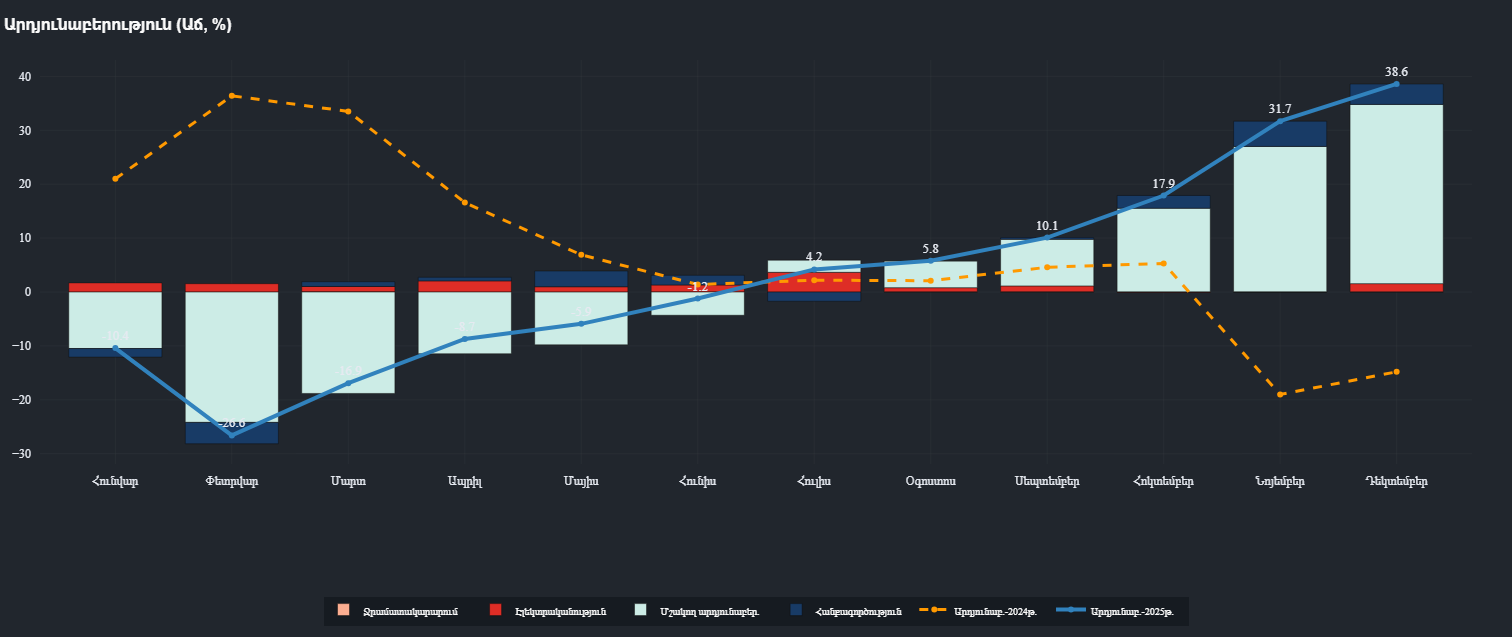
\includegraphics[width=0.8\textwidth]{figures/10_industry_monthly_24_25.png}
    \caption{Monthly Industrial Production (2025)}
    \label{fig:industry_monthly}
\end{figure}

\begin{figure}[H]
    \centering
    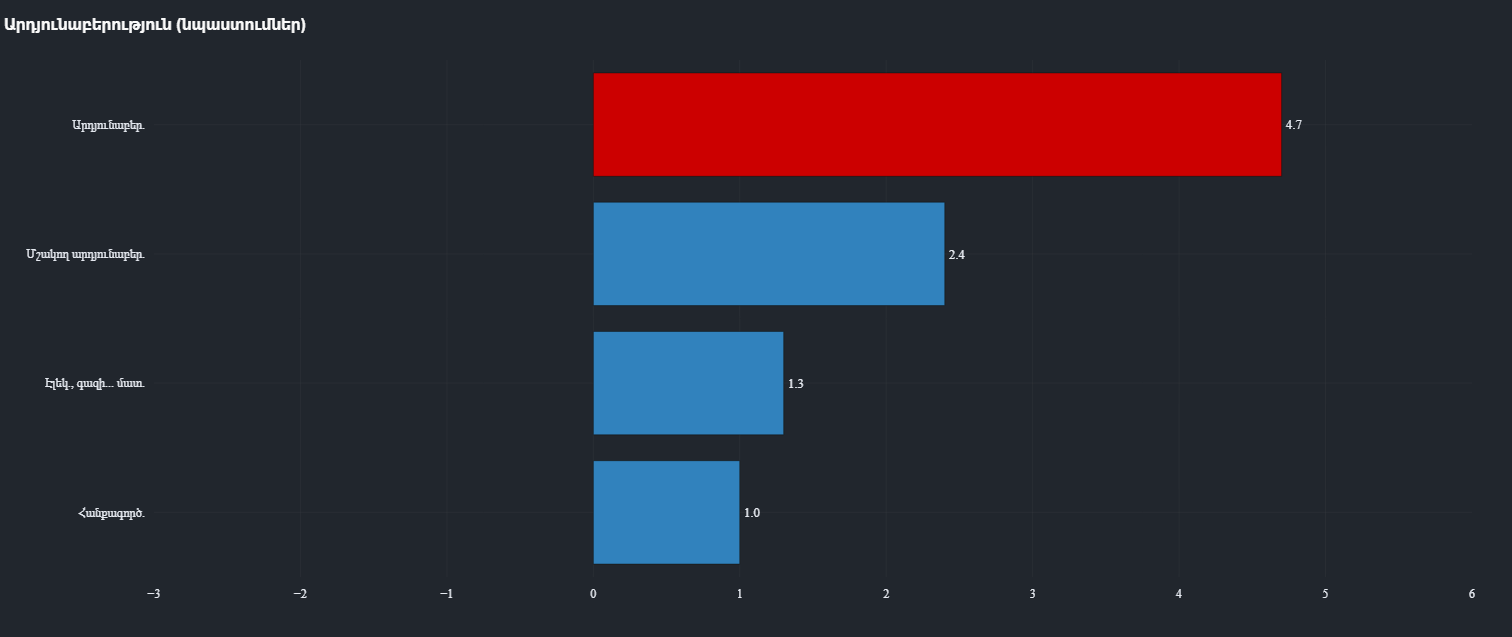
\includegraphics[width=0.8\textwidth]{figures/11_industry_sector_contributions.png}
    \caption{Structural Composition of Industrial Output}
    \label{fig:industry_structure}
\end{figure}

\begin{figure}[H]
    \centering
    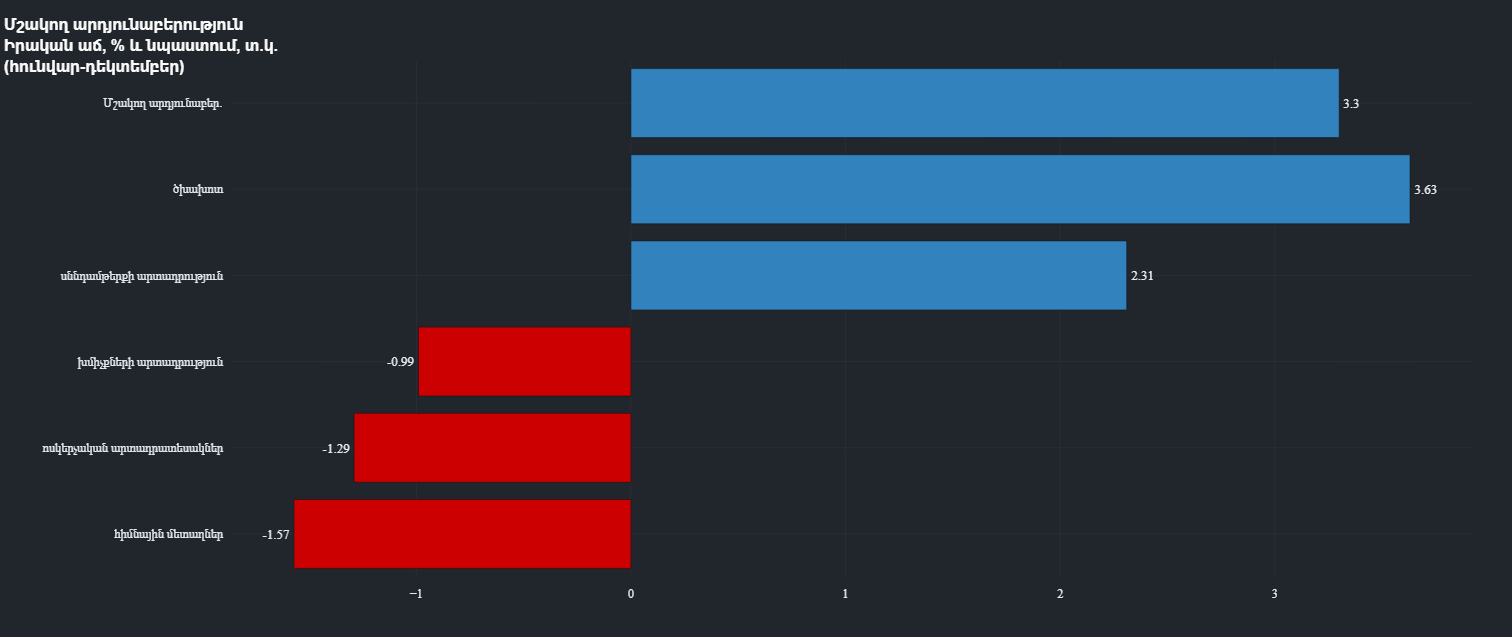
\includegraphics[width=0.8\textwidth]{figures/12_manufacturing_subsectors.png}
    \caption{Growth Rates in Key Manufacturing Subsectors}
    \label{fig:manufacturing}
\end{figure}

Industrial performance should be interpreted as a test of whether growth is becoming more production-based and export-capable. Figure \ref{fig:industry_monthly} captures cyclical momentum; Figure \ref{fig:industry_structure} reveals the weight of major branches; Figure \ref{fig:manufacturing} shows whether subsector growth is concentrated or broad. If mining rebounds while manufacturing remains uneven, the result is resilience without deep structural upgrading. If several manufacturing subsectors strengthen simultaneously, the evidence for diversification becomes much stronger. In this thesis, industry appears more stable than weak, but still less central than construction and services in explaining short-run aggregate acceleration.

\section{Agriculture and Supply-Side Stability}
\begin{figure}[H]
    \centering
    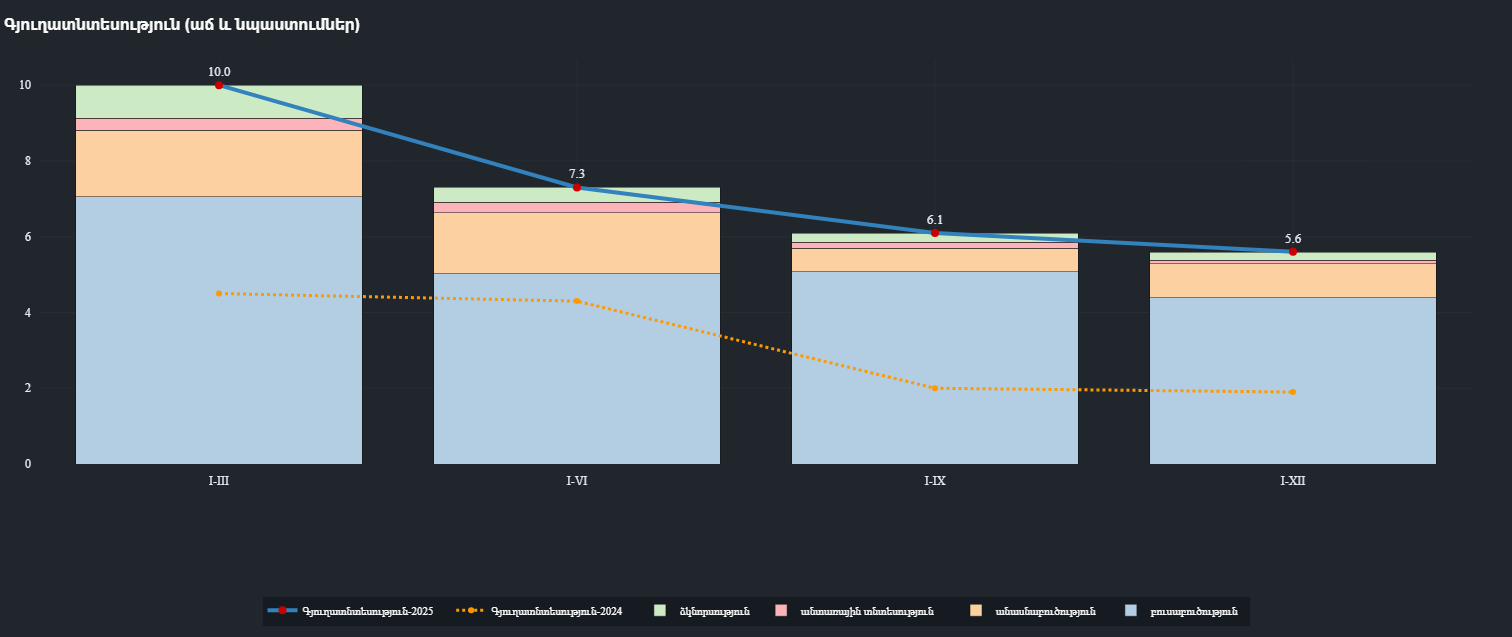
\includegraphics[width=0.8\textwidth]{figures/13_agriculture_cumulative.png}
    \caption{Cumulative Agricultural Production (2025)}
    \label{fig:agri_cumulative}
\end{figure}

\begin{figure}[H]
    \centering
    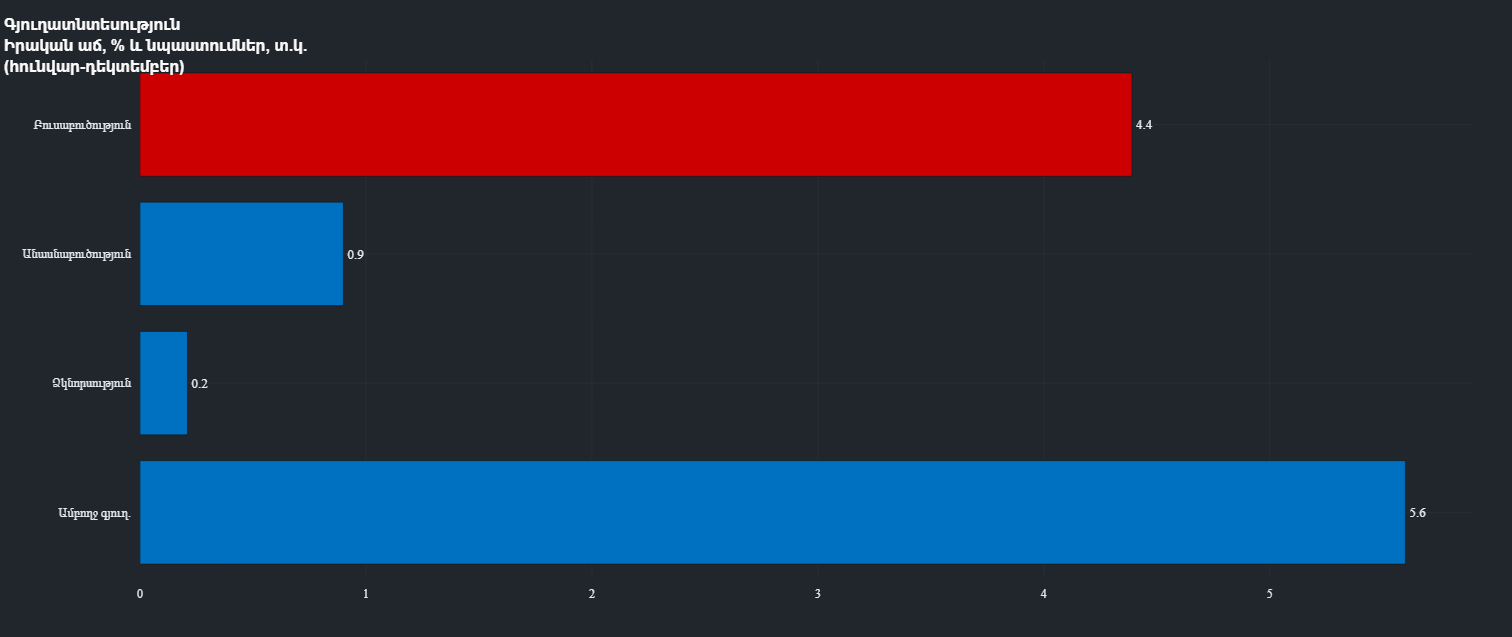
\includegraphics[width=0.8\textwidth]{figures/14_agriculture_sector_contributions.png}
    \caption{Sectoral Distribution of Agricultural Growth}
    \label{fig:agri_sectors}
\end{figure}

Agriculture is not the dominant source of Armenian GDP growth, but it remains important for inflation, rural incomes, and supply-side stability. Figure \ref{fig:agri_cumulative} shows the general trend, while Figure \ref{fig:agri_sectors} indicates whether gains are narrowly concentrated or distributed across subsectors. In analytical terms, stable agricultural performance reduces the probability that low inflation is achieved solely through weak demand or imported disinflation. It also matters for the inclusiveness of growth. A growth model that is too urban and too construction-heavy may raise GDP without diffusing benefits geographically. Agriculture therefore functions in this thesis as a stabilizing rather than leading sector.

\section{Construction, Real Estate, and the Risk of Imbalance}
\begin{figure}[H]
    \centering
    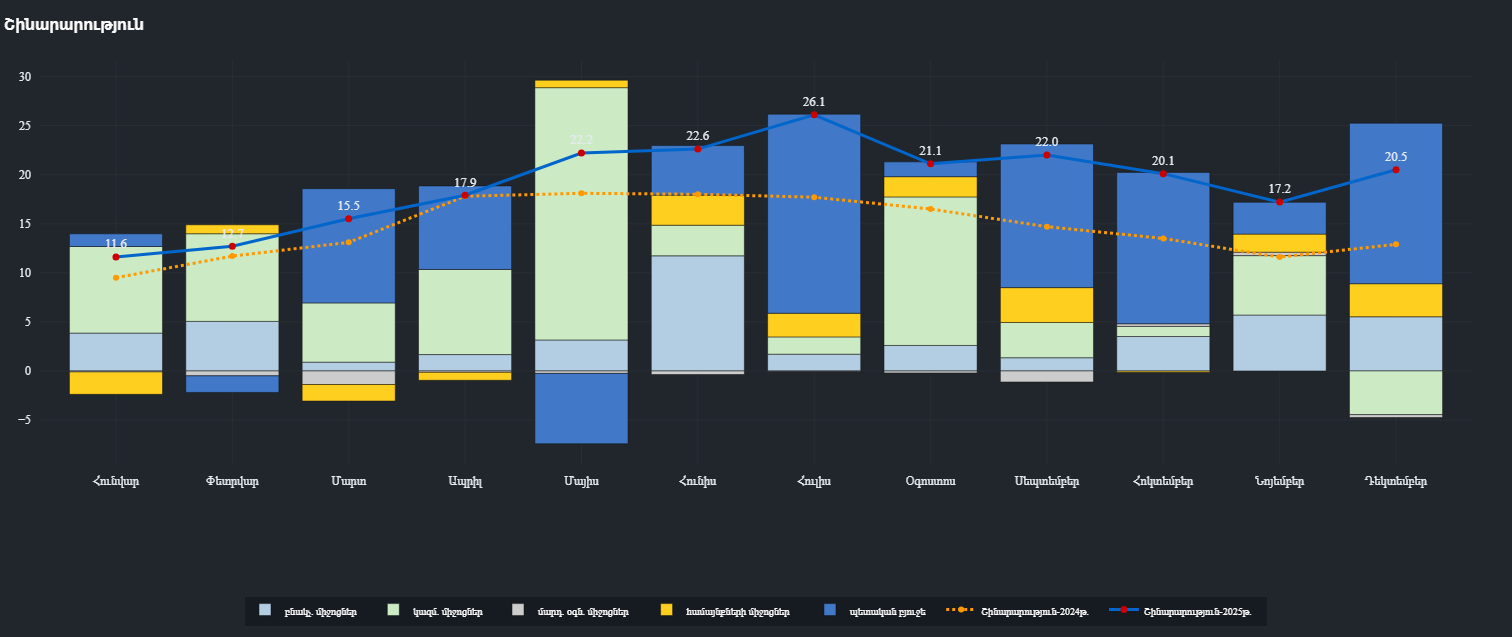
\includegraphics[width=0.8\textwidth]{figures/15_construction_monthly_24_25.png}
    \caption{Construction Sector Growth: Monthly Indices}
    \label{fig:construction_monthly}
\end{figure}

\begin{figure}[H]
    \centering
    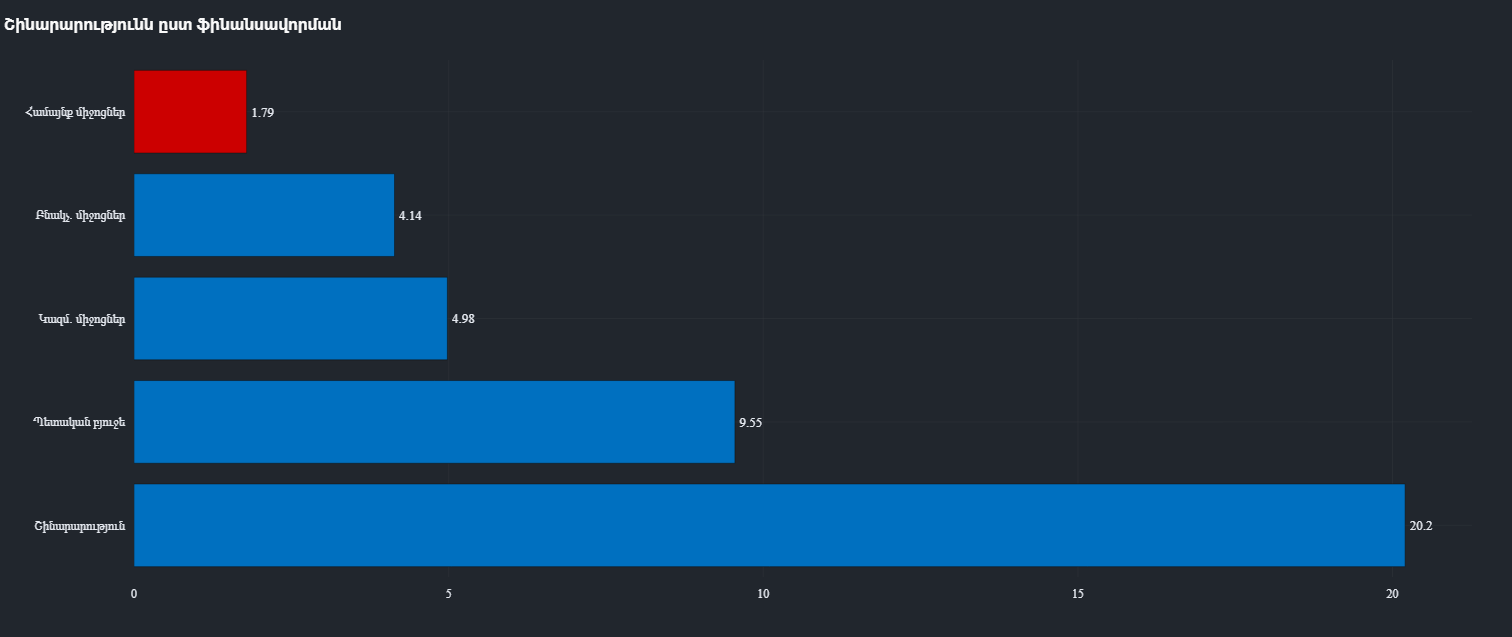
\includegraphics[width=0.8\textwidth]{figures/16_construction_funding_sources.png}
    \caption{Diversification of Construction Funding Sources: State vs Private}
    \label{fig:construction_funding}
\end{figure}

\begin{figure}[H]
    \centering
    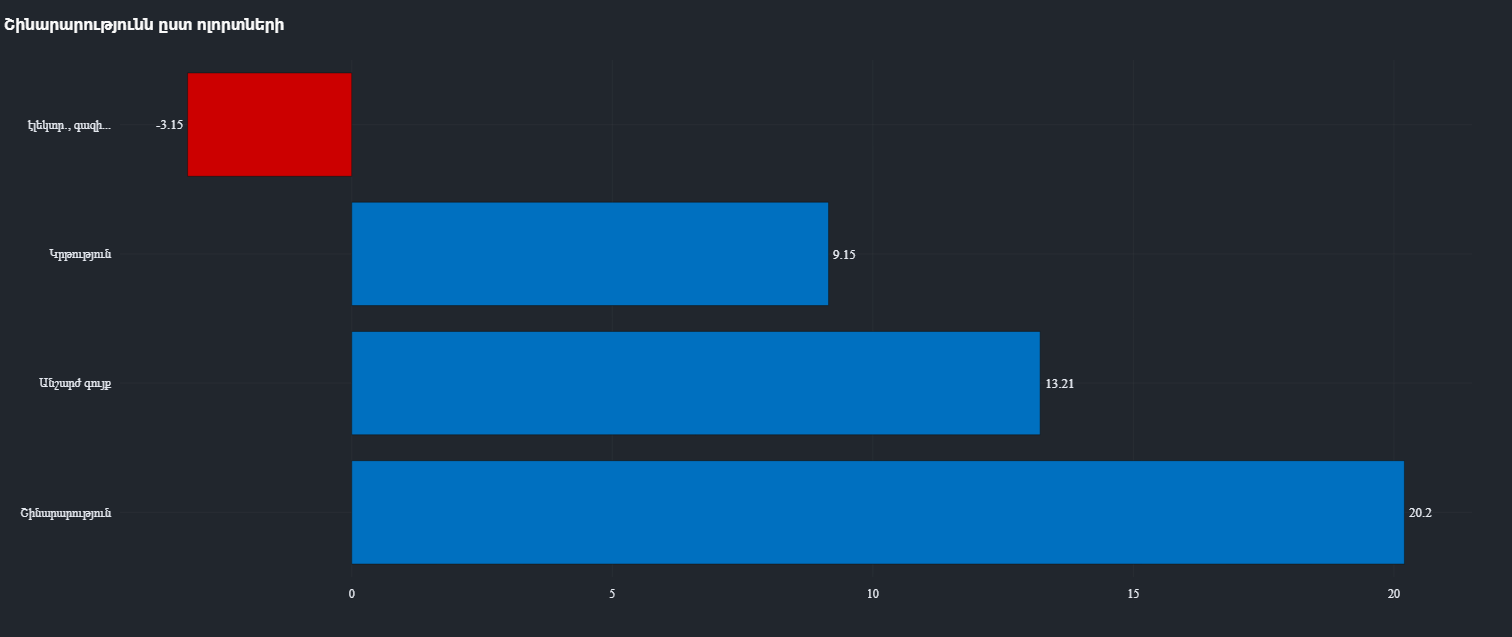
\includegraphics[width=0.8\textwidth]{figures/17_construction_by_sector.png}
    \caption{Construction Output by Targeted Economic Sector}
    \label{fig:construction_by_sector}
\end{figure}

\begin{figure}[H]
    \centering
    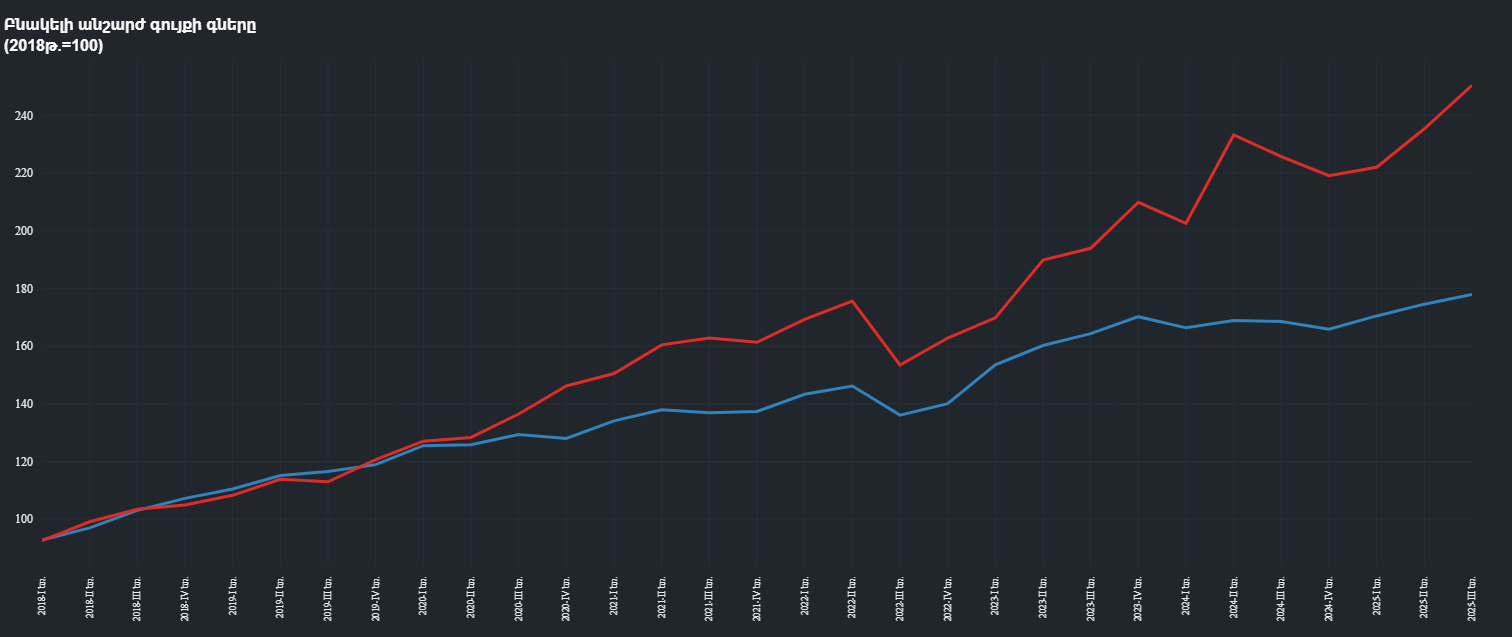
\includegraphics[width=0.8\textwidth]{figures/18_real_estate_prices.png}
    \caption{Real Estate Price Index: Apartments vs Private Houses}
    \label{fig:re_prices}
\end{figure}

\begin{figure}[H]
    \centering
    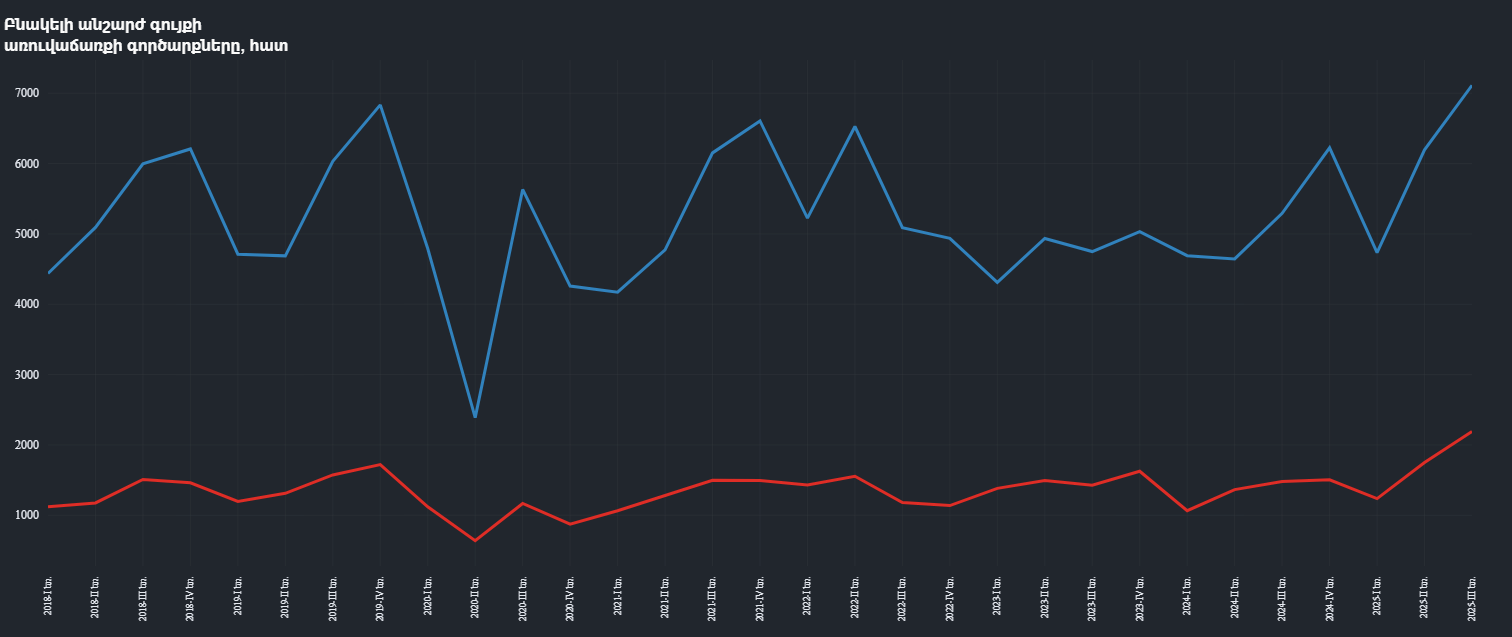
\includegraphics[width=0.8\textwidth]{figures/19_real_estate_transactions.png}
    \caption{Volume of Real Estate Transactions: National Overview}
    \label{fig:re_trans}
\end{figure}

\begin{figure}[H]
    \centering
    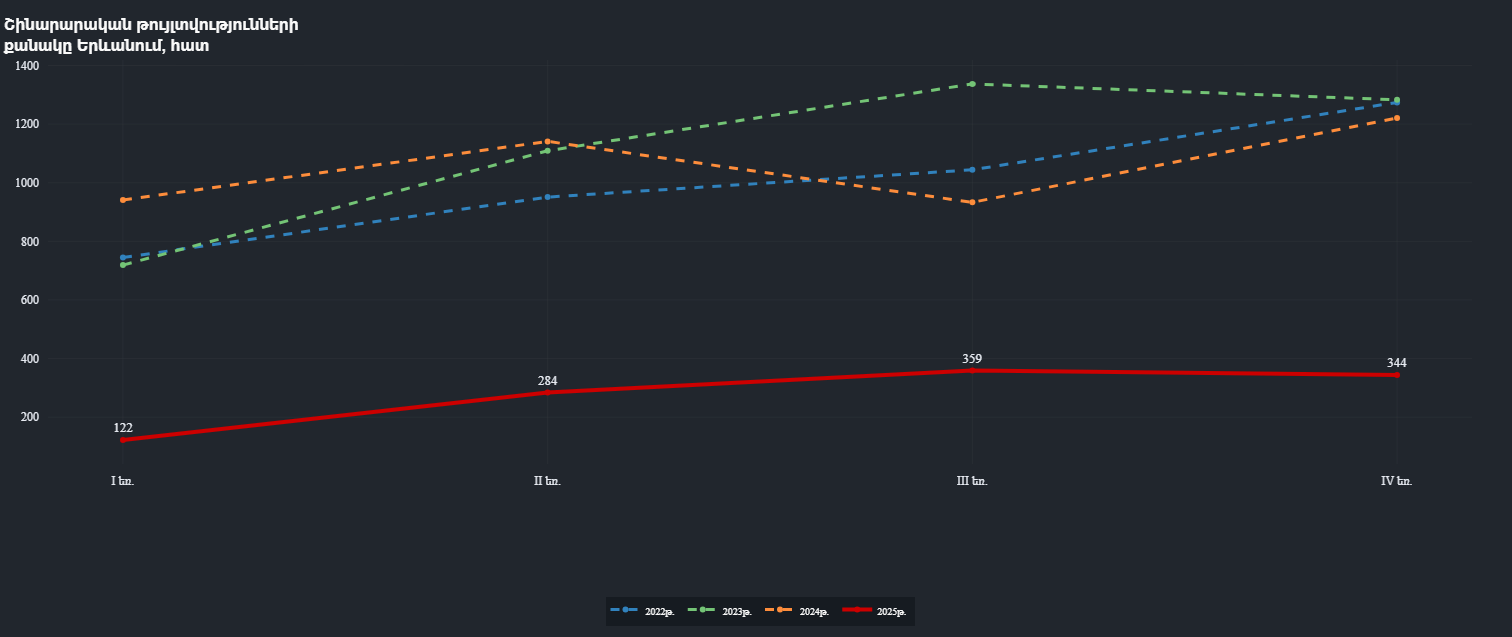
\includegraphics[width=0.8\textwidth]{figures/20_construction_permits_yerevan.png}
    \caption{Yerevan Construction Permits: A Leading Indicator for 2025}
    \label{fig:permits_yerevan}
\end{figure}

Construction is the most important sector in the thesis and also the main source of concern. Figures \ref{fig:construction_monthly}--\ref{fig:permits_yerevan} suggest that the sector was not merely expanding, but shaping the broader macroeconomic environment through investment, employment, housing demand, and bank credit. The analytical question is whether this represents healthy capital formation or concentration risk. A diversified funding structure would reduce vulnerability, but persistent price increases, elevated transaction activity, and strong permit issuance may also indicate overheating in urban real estate. Therefore, construction should be interpreted as both a growth engine and a fragility channel. If aggregate GDP is increasingly tied to this sector, then the apparent strength of Armenia's economy may overstate its balance.

\chapter{Labor Market, Demographics, and Social Dynamics}
\section{Employment and the ICT Shift}
\begin{figure}[H]
    \centering
    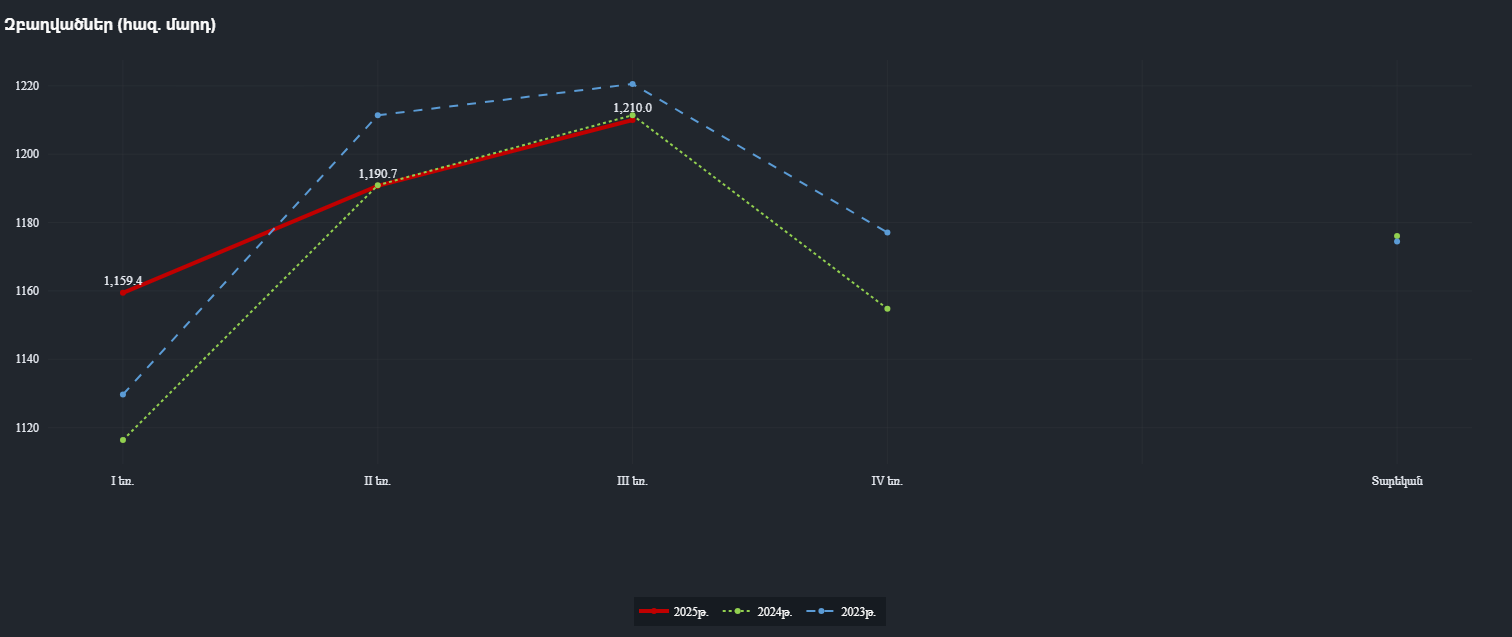
\includegraphics[width=0.8\textwidth]{figures/21_employment_quarterly.png}
    \caption{Total Employment: Quarterly Trends (Thousands)}
    \label{fig:employment_q}
\end{figure}

\begin{figure}[H]
    \centering
    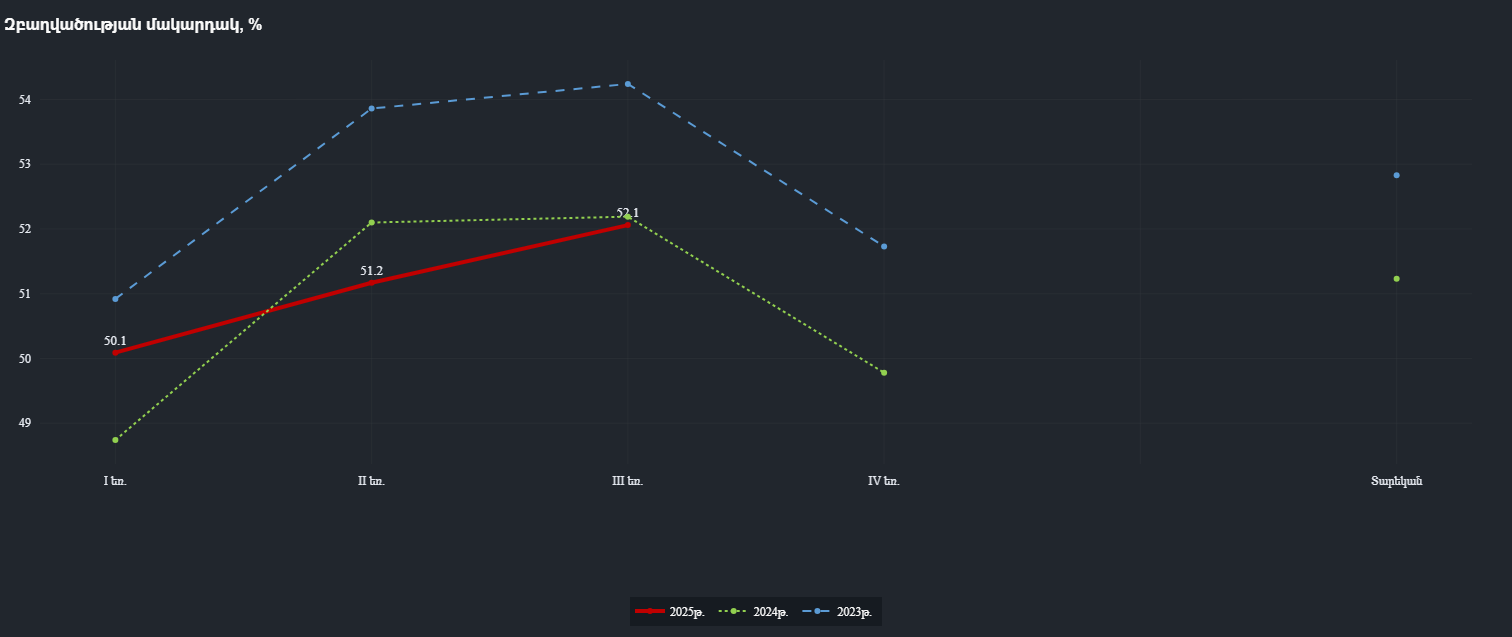
\includegraphics[width=0.8\textwidth]{figures/22_employment_rate.png}
    \caption{Employment Rate (\%) Performance}
    \label{fig:emp_rate}
\end{figure}

\begin{figure}[H]
    \centering
    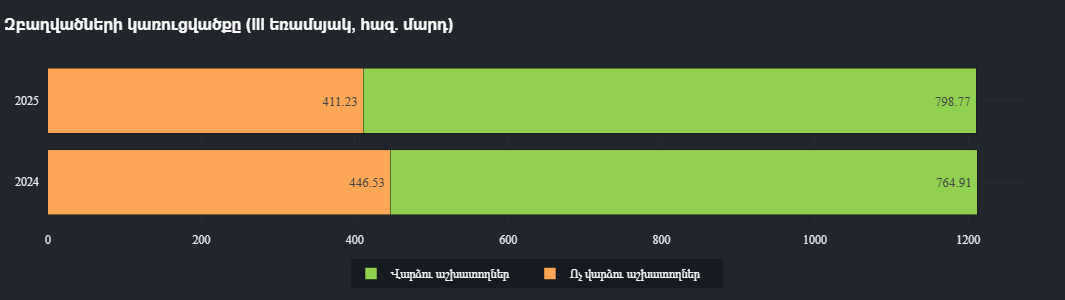
\includegraphics[width=0.8\textwidth]{figures/23_employment_structure.png}
    \caption{Labor Market Structure: Wage Employees vs Self-Employed}
    \label{fig:emp_structure}
\end{figure}

Labor indicators help determine whether Armenia's growth translated into formalization and productive job creation. Figures \ref{fig:employment_q} and \ref{fig:emp_rate} indicate whether labor demand remained robust, while Figure \ref{fig:emp_structure} reveals whether employment shifted toward wage-based forms associated with formal-sector expansion. This matters because the ICT story is economically meaningful only if it supports durable employment, wage growth, and productivity rather than isolated firm-level success. The thesis interprets the labor data as evidence of tightening conditions, but not as proof that all sectors are becoming equally productive. The transition toward more formal employment is a positive sign; the challenge is whether high-value job creation is broad enough to absorb labor outside the main urban and service centers.

\section{Unemployment and Labor-Market Tightness}
\begin{figure}[H]
    \centering
    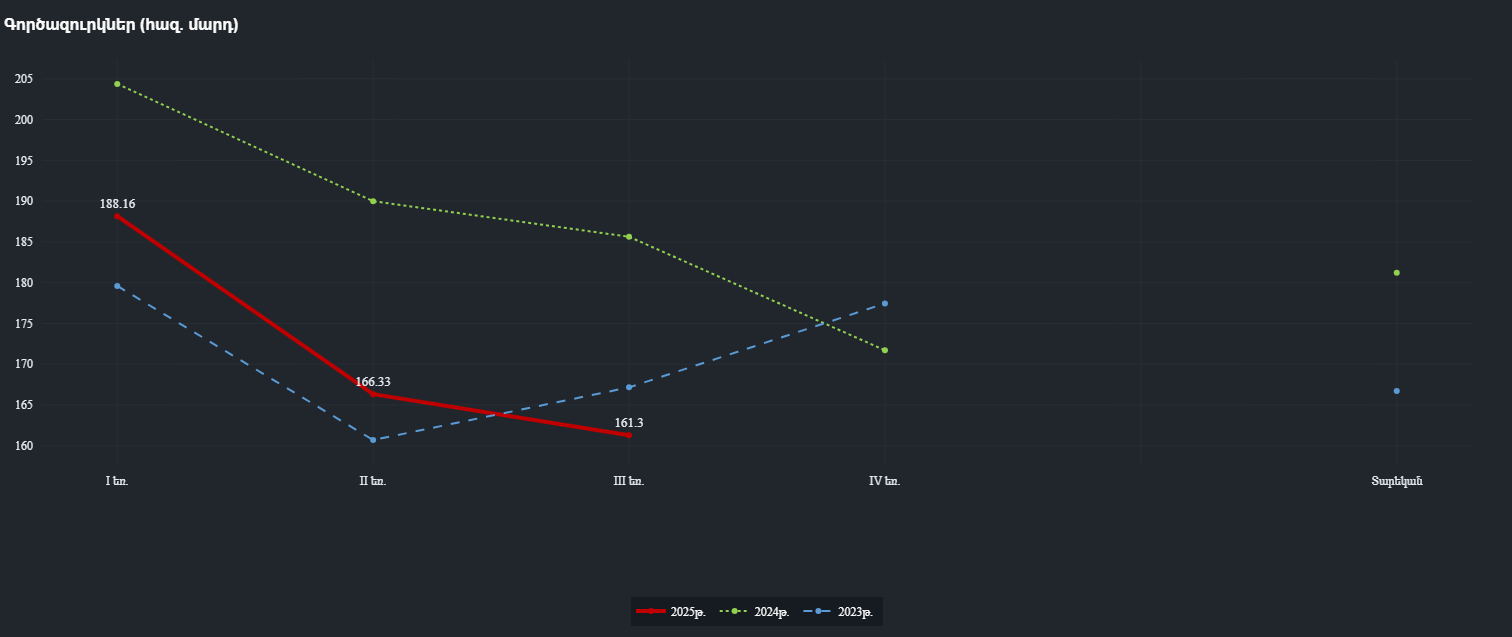
\includegraphics[width=0.8\textwidth]{figures/24_unemployment_count.png}
    \caption{Total Unemployed Count (Thousands)}
    \label{fig:unemp_count}
\end{figure}

\begin{figure}[H]
    \centering
    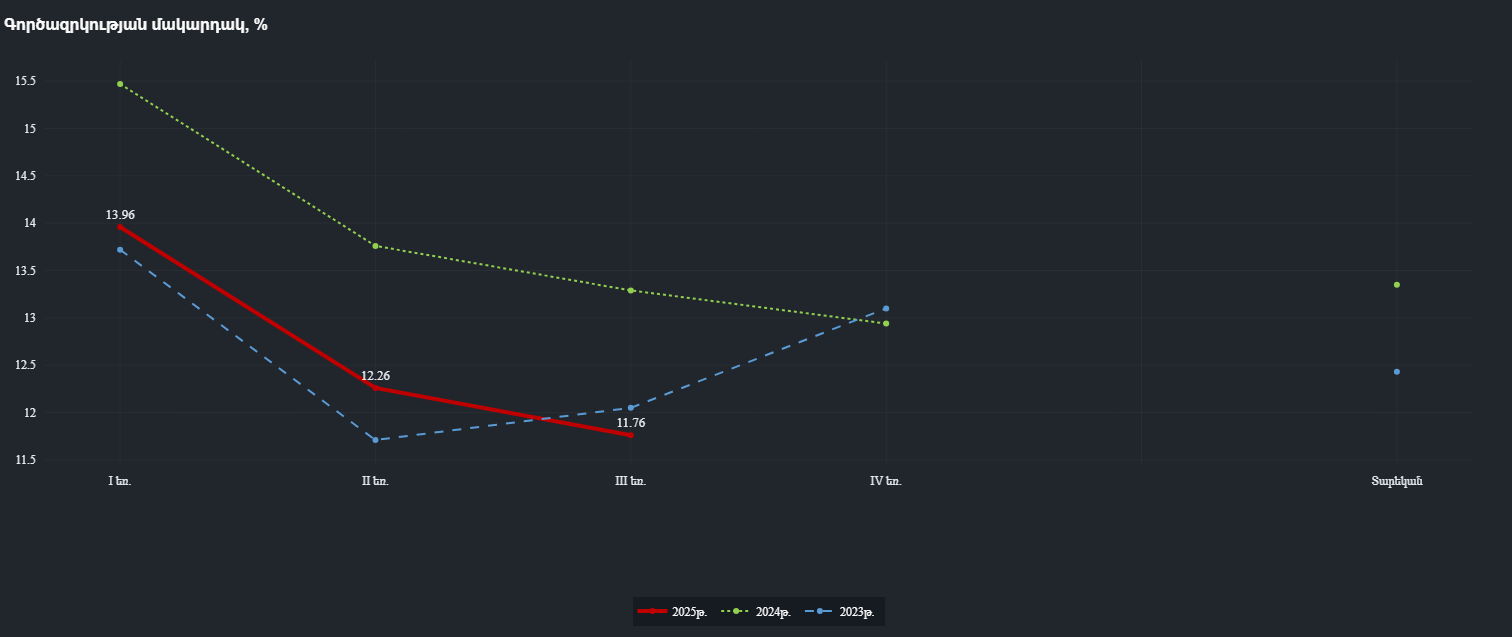
\includegraphics[width=0.8\textwidth]{figures/25_unemployment_rate.png}
    \caption{Unemployment Rate Dynamics (2025)}
    \label{fig:unemployment_rate}
\end{figure}

\begin{figure}[H]
    \centering
    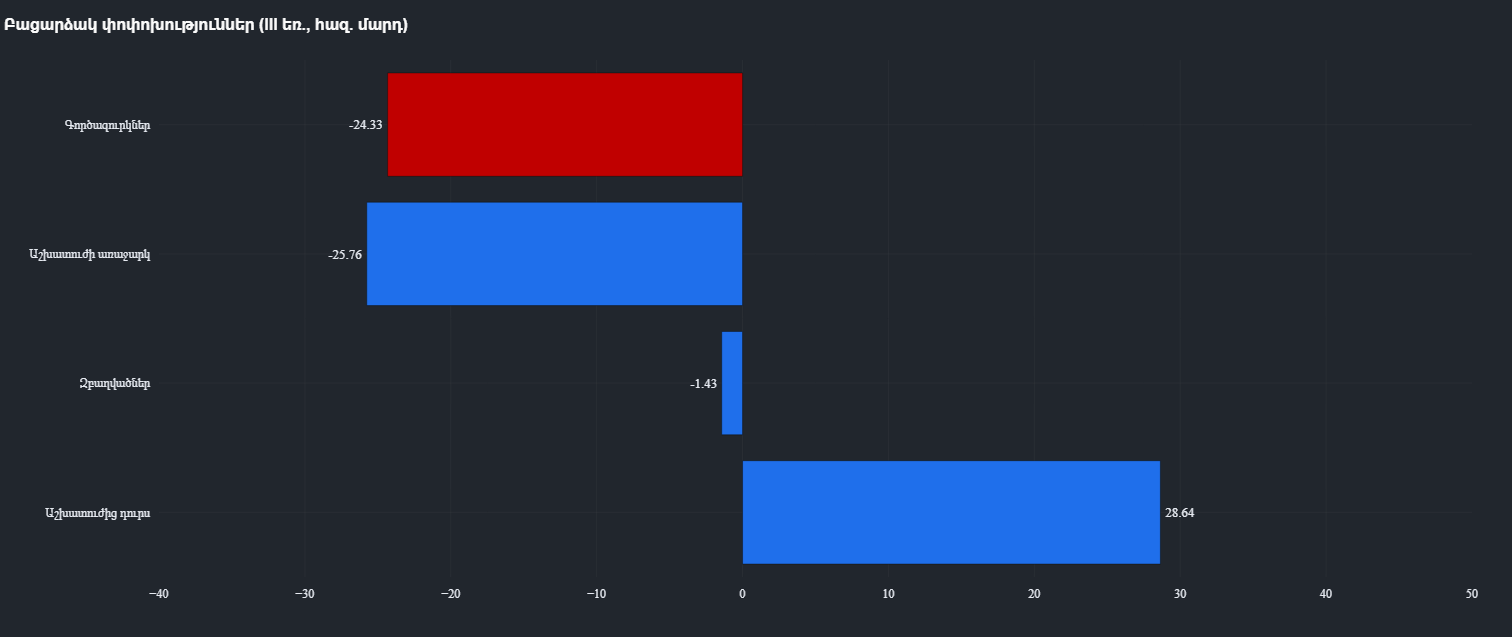
\includegraphics[width=0.8\textwidth]{figures/26_labor_market_changes.png}
    \caption{Analytical Summary of Labor Market Flows}
    \label{fig:labor_flows}
\end{figure}

\begin{figure}[H]
    \centering
    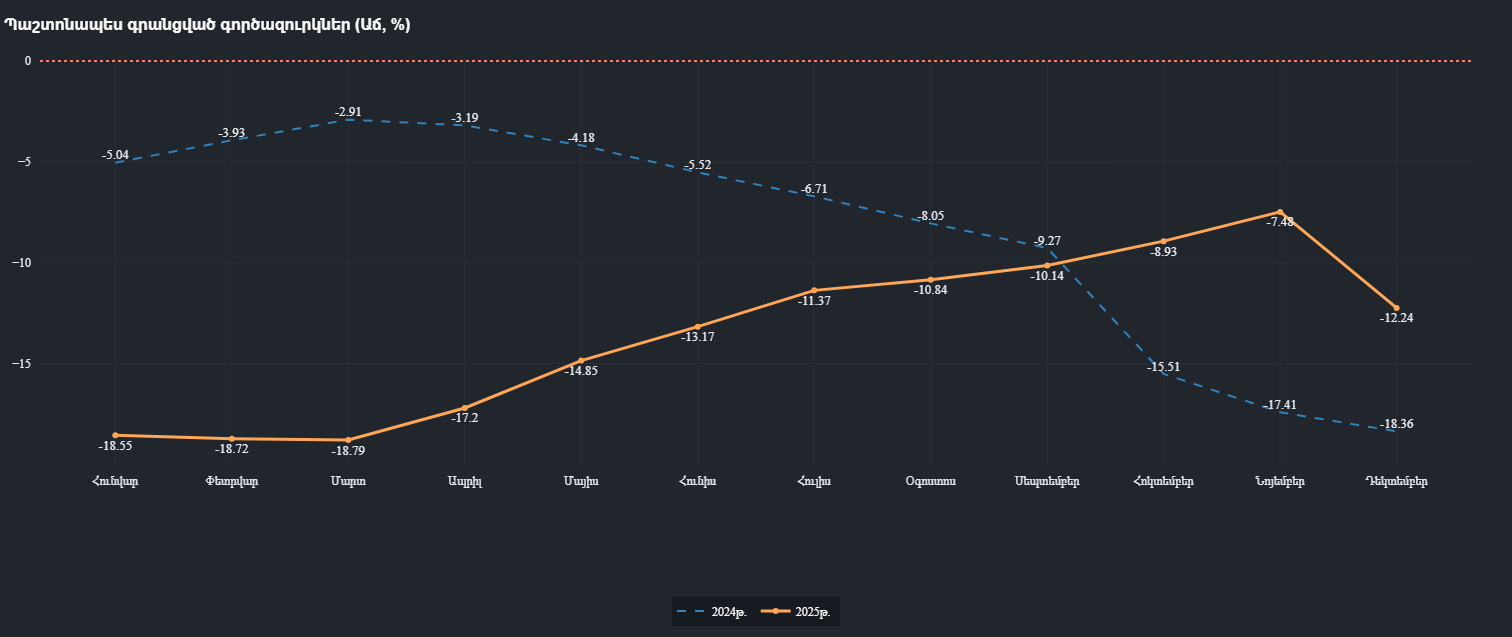
\includegraphics[width=0.8\textwidth]{figures/27_registered_unemployed_growth.png}
    \caption{Year-on-Year Growth of Registered Unemployed}
    \label{fig:registered_unemp}
\end{figure}

Falling unemployment can indicate genuine labor-market improvement, but in Armenia it must be interpreted together with migration, participation, and skills availability. Figures \ref{fig:unemp_count}--\ref{fig:registered_unemp} are therefore read as a set. If unemployment declines while labor demand rises and formal employment expands, then the macro signal is clearly positive. If unemployment declines while labor-force participation weakens or registered unemployment behaves differently from survey-based measures, then the interpretation is more complex. The thesis reads current dynamics as evidence of tightening labor conditions, with an emerging risk that labor shortages, especially in skilled occupations, could limit further expansion in ICT, advanced services, and parts of manufacturing.

\section{Migration, Labor Supply, and Demographic Dynamics}
\begin{figure}[H]
    \centering
    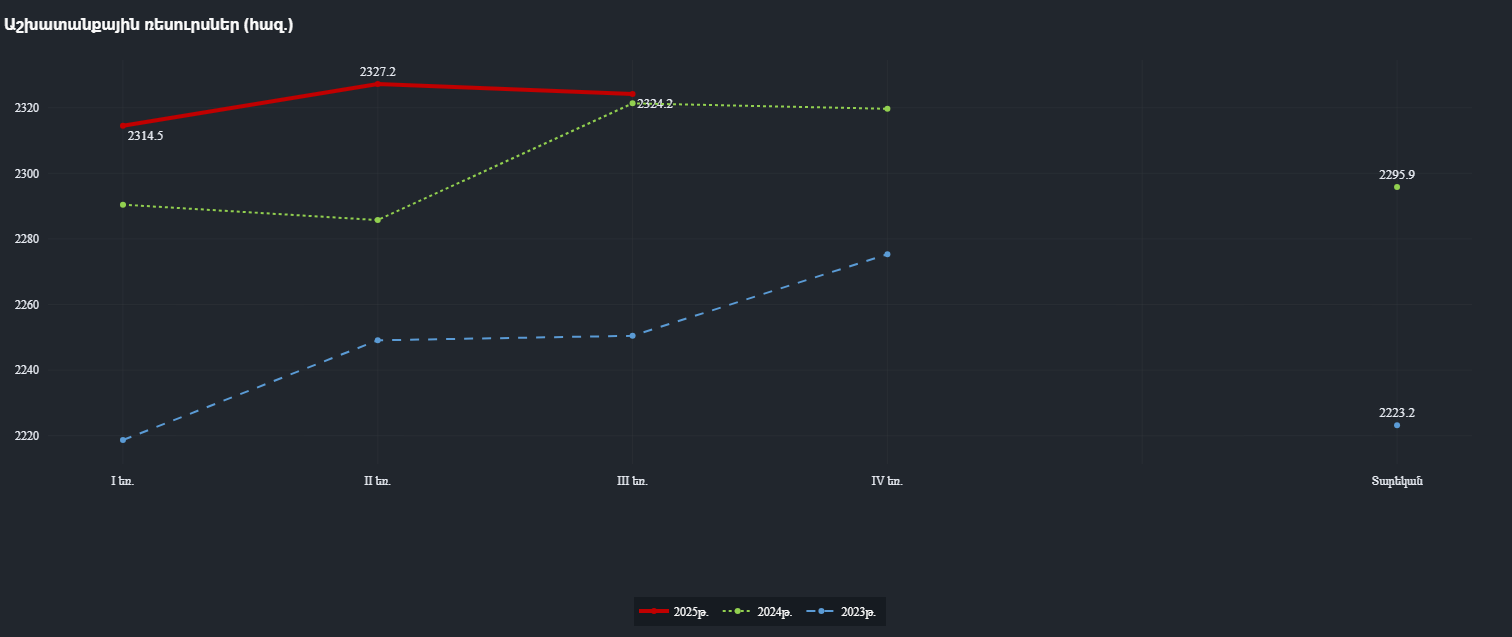
\includegraphics[width=0.8\textwidth]{figures/28_labor_resources.png}
    \caption{Evolution of Total Labor Resources}
    \label{fig:labor_resources}
\end{figure}

\begin{figure}[H]
    \centering
    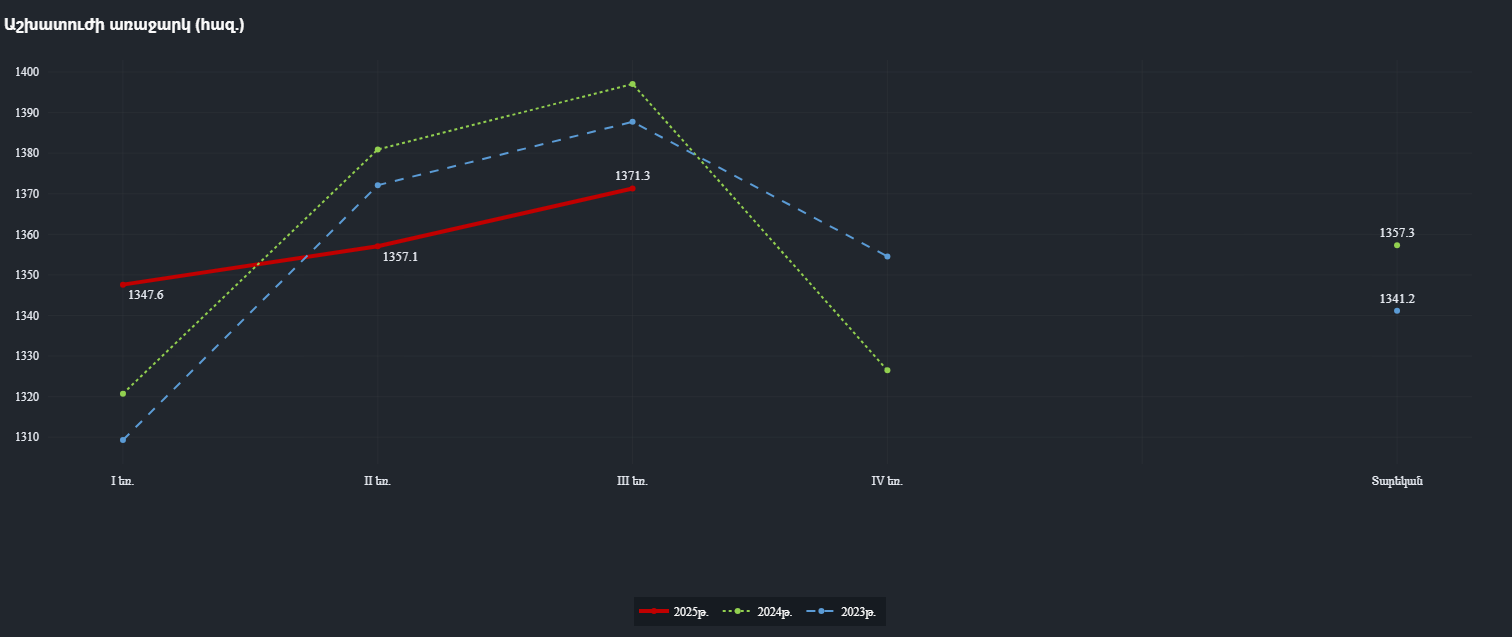
\includegraphics[width=0.8\textwidth]{figures/29_labor_supply.png}
    \caption{Active Labor Supply Trends}
    \label{fig:labor_supply}
\end{figure}

\begin{figure}[H]
    \centering
    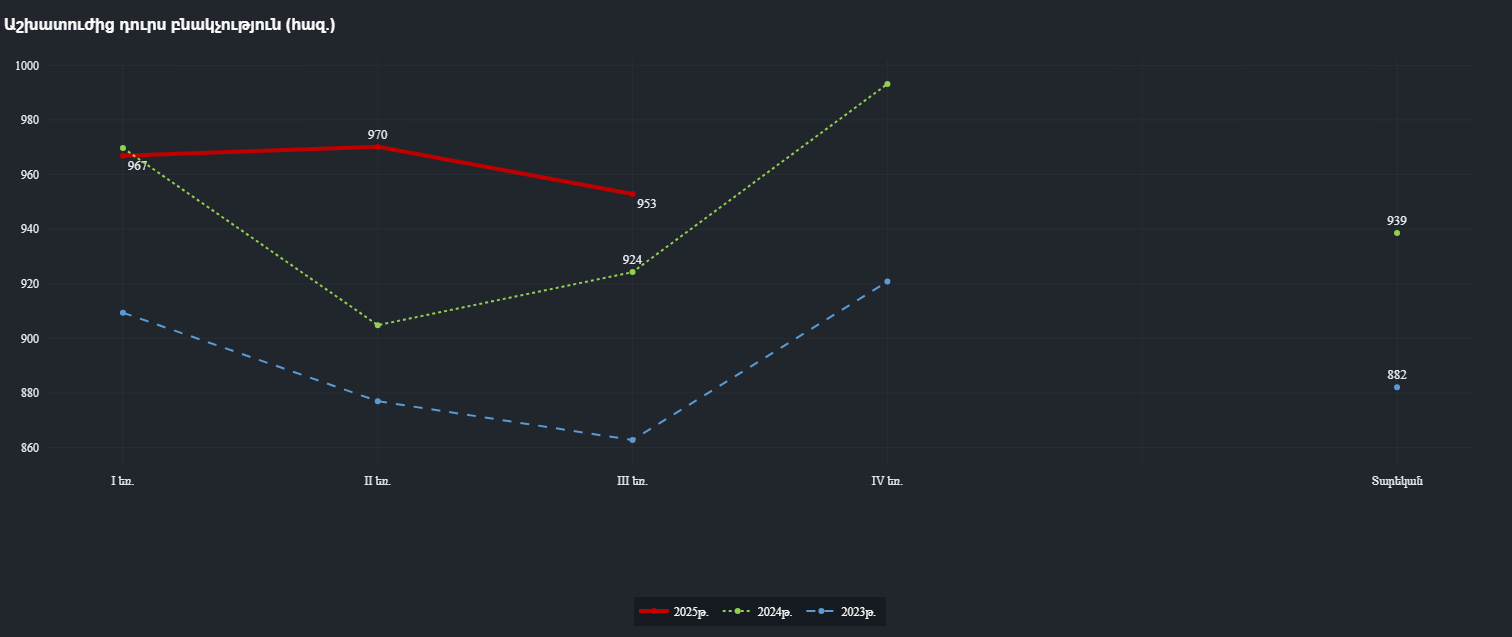
\includegraphics[width=0.8\textwidth]{figures/30_outside_labor_force.png}
    \caption{Population Outside the Labor Force (Non-Active)}
    \label{fig:outside_labor}
\end{figure}

\begin{figure}[H]
    \centering
    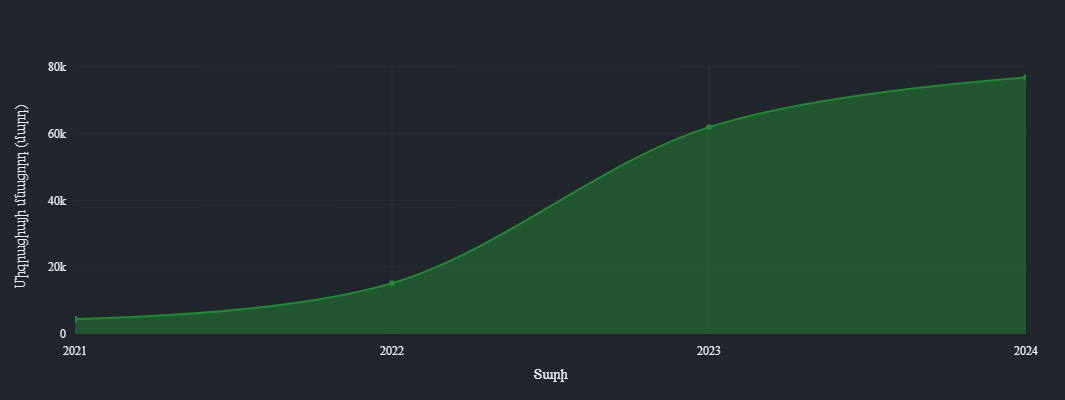
\includegraphics[width=0.8\textwidth]{figures/40_migration_balance.png}
    \caption{Net Migration Balance: Longitudinal View (2021-2024)}
    \label{fig:migration}
\end{figure}

Migration has macroeconomic significance in Armenia because it affects labor supply, housing demand, services consumption, and fiscal needs simultaneously. Figures \ref{fig:labor_resources}--\ref{fig:migration} suggest that demographic dynamics contributed to the economy's resilience, but the effect should not be romanticized. A positive migration balance can temporarily support demand and labor availability, yet it can also intensify pressure on housing, public services, and urban infrastructure. The main analytical conclusion is that migration strengthened short-run economic capacity, but it did not eliminate the need for deeper productivity growth and better labor allocation.

\section{Wages and Purchasing Power}
\begin{figure}[H]
    \centering
    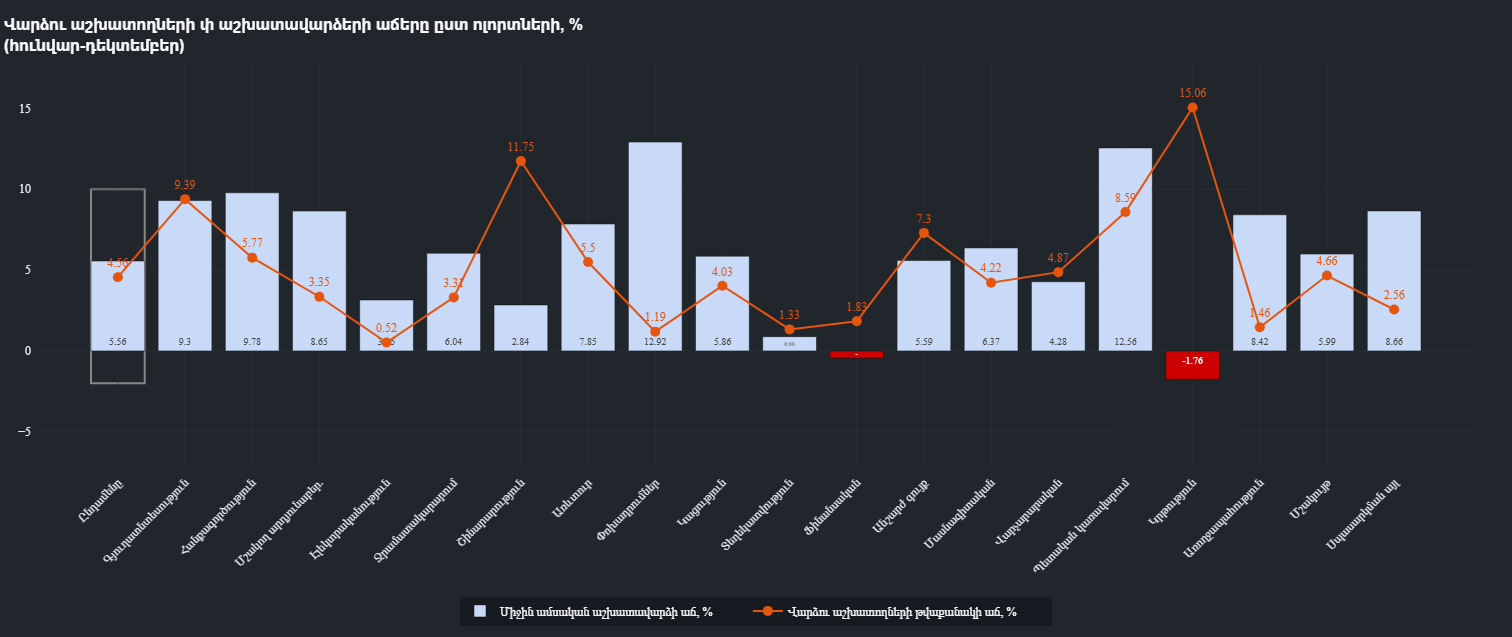
\includegraphics[width=0.8\textwidth]{figures/31_wage_headcount_by_sector.png}
    \caption{Nominal Wage Growth vs Headcount Changes by Sector}
    \label{fig:wages_headcount}
\end{figure}

Figure \ref{fig:wages_headcount} is valuable because it links sectoral labor demand to income dynamics. Rapid wage growth in sectors with expanding headcount usually signals strong demand and possible productivity gains, but rapid wage growth with weak headcount growth may instead reflect scarcity of specialized labor. In Armenia's case, the combination of construction and ICT wage dynamics reinforces the thesis's central argument: the economy was expanding, but the benefits and pressures of that expansion were concentrated in a limited number of sectors. This supports the view that labor-market tightening was real, while also highlighting the risk of inequality between dynamic urban sectors and the rest of the economy.

\chapter{Macroeconomic Stability, Fiscal Policy, and Financial Exposure}
\section{Inflation and Monetary Conditions}
\begin{figure}[H]
    \centering
    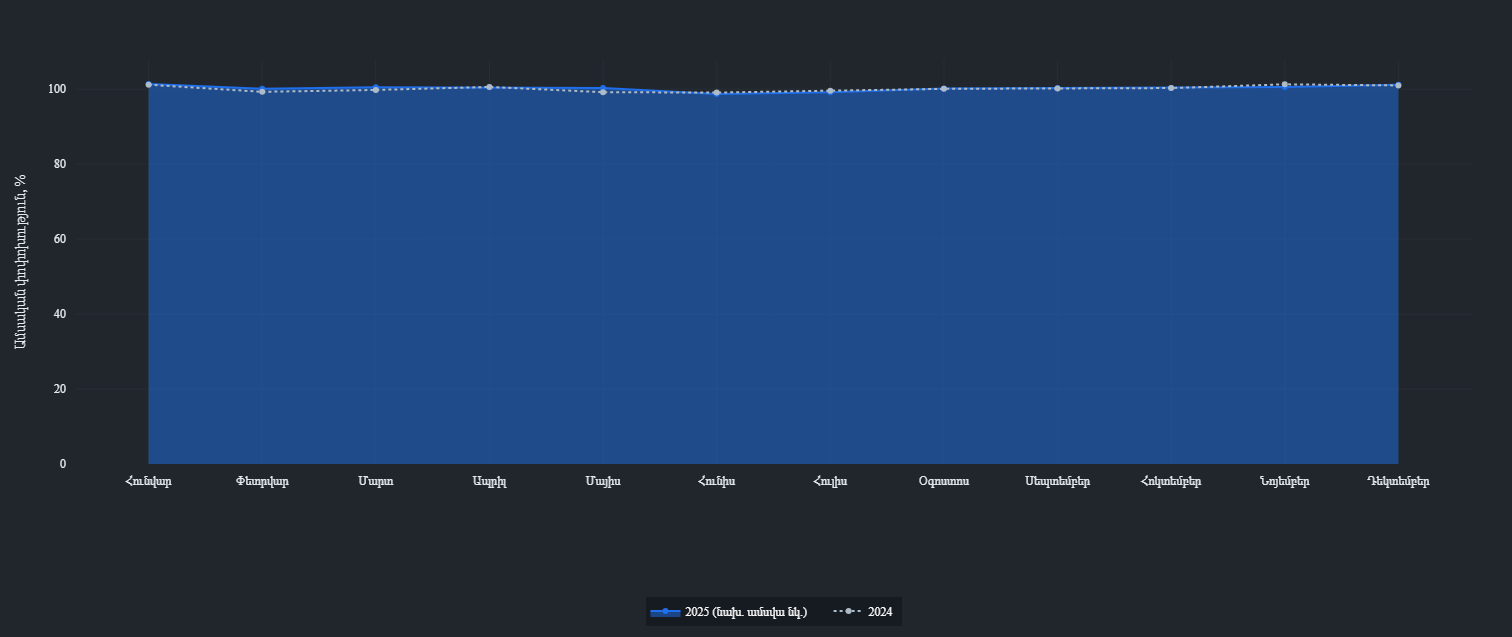
\includegraphics[width=0.8\textwidth]{figures/34_monthly_cpi.png}
    \caption{Consumer Price Index (CPI) Stability (Monthly)}
    \label{fig:cpi}
\end{figure}

Inflation performance is a key test of whether fast growth remained manageable. Figure \ref{fig:cpi} suggests that price pressures were relatively contained compared with the scale of domestic expansion. This is analytically important because it indicates that strong growth did not automatically translate into generalized overheating. However, low inflation alone should not be treated as proof of macroeconomic perfection. Imported disinflation, exchange-rate effects, and sector-specific supply conditions may all contribute to headline price stability. The thesis therefore interprets subdued inflation as supportive evidence of stability, but not as a sufficient argument against underlying imbalances elsewhere in the economy.\cite{cbaImpl2025,cbaMPR2025Q1}

\section{Fiscal Position and the Quality of Public Demand}
\begin{figure}[H]
    \centering
    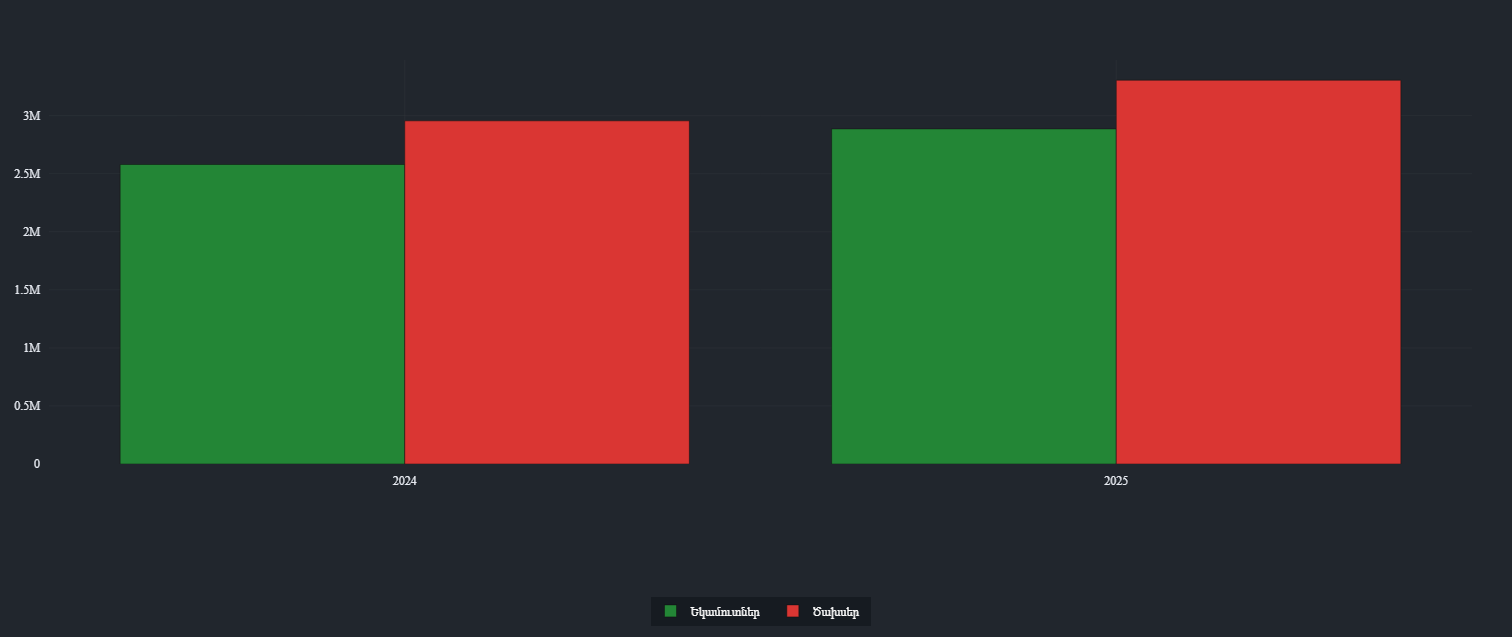
\includegraphics[width=0.8\textwidth]{figures/36_state_budget_revenue_expenditure.png}
    \caption{State Budget Revenues vs Expenditures (2025)}
    \label{fig:budget}
\end{figure}

Fiscal developments matter for two reasons. First, the budget affects aggregate demand directly through public investment and social spending. Second, a construction-led economy can become more dependent on public capital expenditure than headline GDP figures initially reveal. Figure \ref{fig:budget} therefore should be read not merely as an accounting comparison between revenues and expenditures, but as evidence on the sustainability of the current growth pattern. If spending rises faster than revenue for several years, fiscal support may be stabilizing in the short run while increasing medium-term debt and financing pressure. The quality of expenditure is thus as important as its scale.\cite{minfinBudget,wbPER2023}

\section{Banking Exposure and Credit Concentration}
\begin{figure}[H]
    \centering
    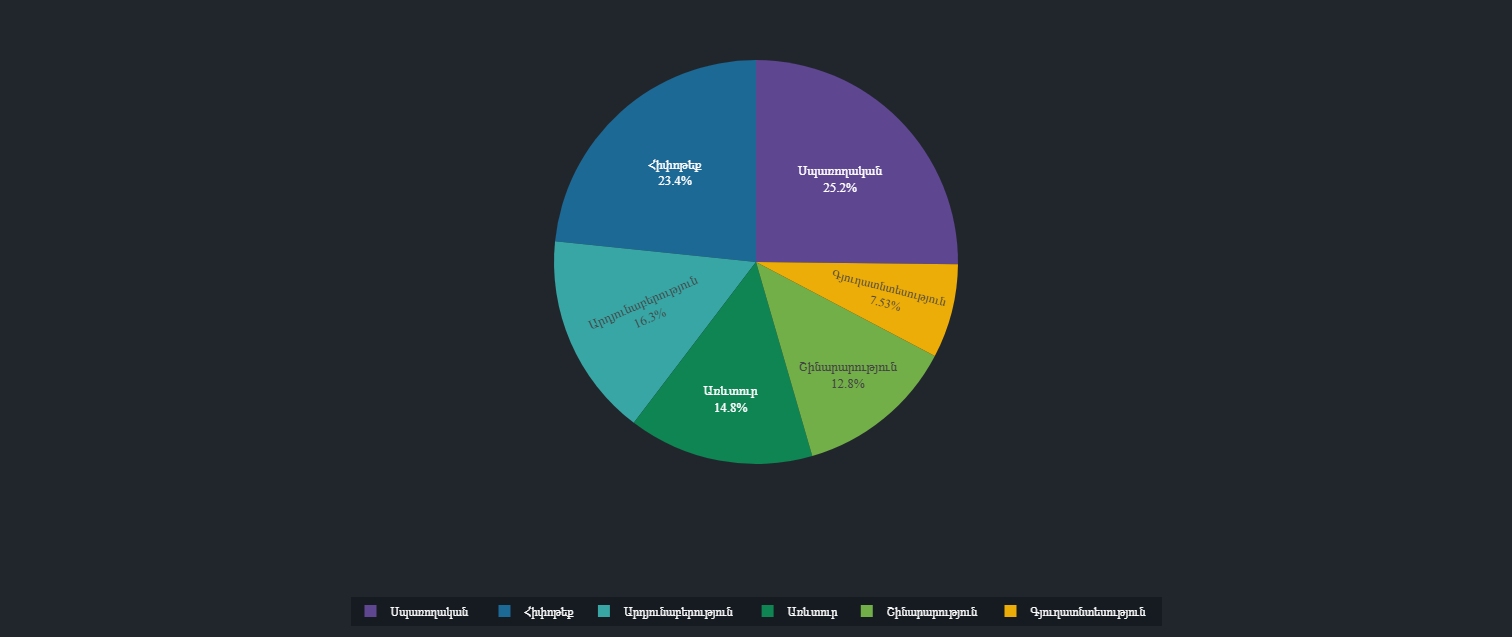
\includegraphics[width=0.8\textwidth]{figures/37_loan_structure_sector.png}
    \caption{Loan Portfolio Distribution by Economic Sector}
    \label{fig:loans}
\end{figure}

Banking-system resilience cannot be evaluated from profitability alone. Figure \ref{fig:loans} is important because it shows sector concentration in the loan book. If credit is disproportionately allocated to construction, mortgages, or consumption-related activities, then the financial system becomes more exposed to a reversal in the same sectors currently driving growth. In that case, the banking sector amplifies the economic cycle instead of merely financing it. The thesis therefore treats loan concentration as a transmission channel of macroeconomic risk, especially when read together with real-estate price growth and permit activity.\cite{imfCR24348,cbaMPR2025Q1}

\section{Trade, Utilities, Regional Output, and the IT Base}
\begin{figure}[H]
    \centering
    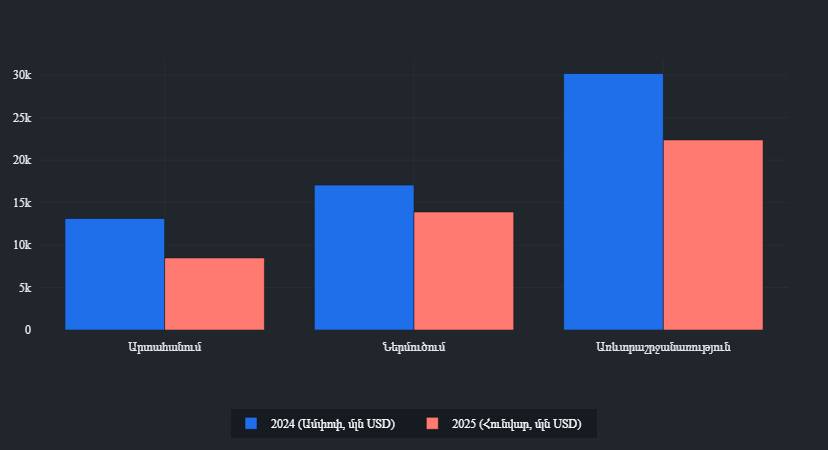
\includegraphics[width=0.8\textwidth]{figures/32_external_trade_comparative.png}
    \caption{External Trade Balance: Exports and Imports Comparison}
    \label{fig:external_trade}
\end{figure}

\begin{figure}[H]
    \centering
    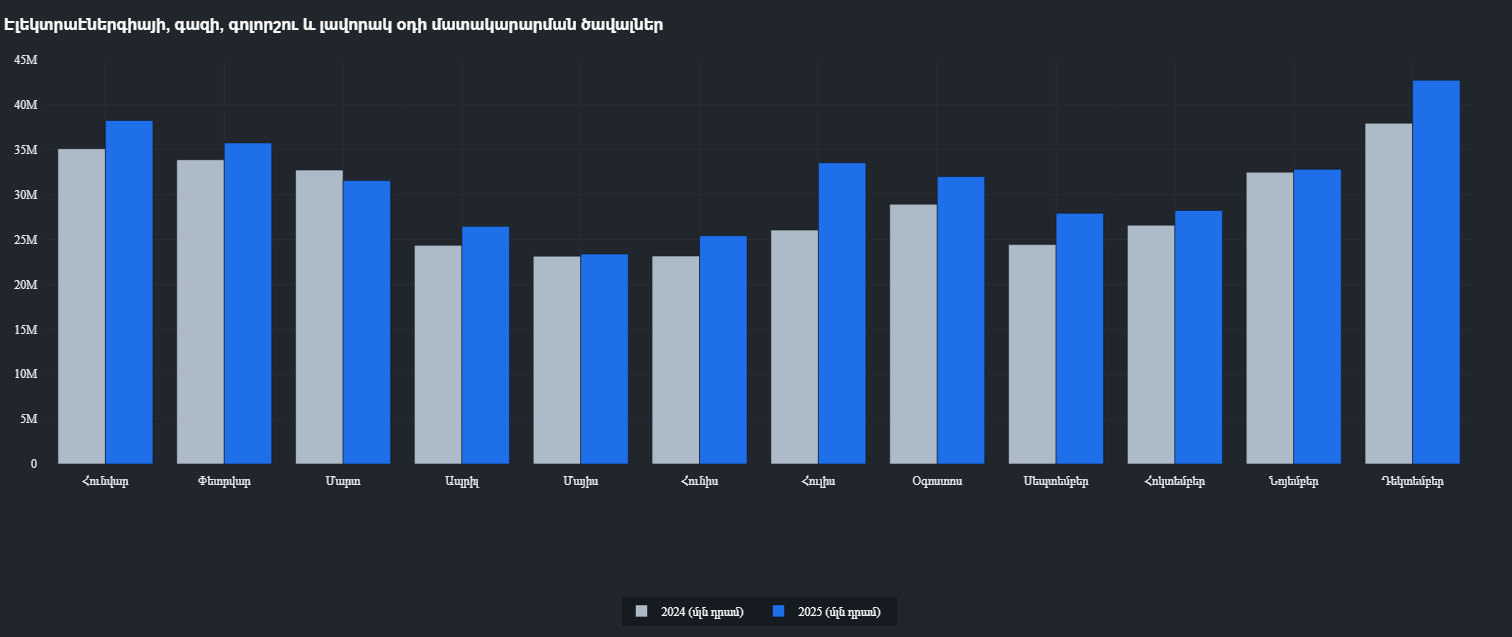
\includegraphics[width=0.8\textwidth]{figures/35_utility_production_monthly.png}
    \caption{Electricity, Gas, and Steam Supply: Monthly Production}
    \label{fig:utilities}
\end{figure}

\begin{figure}[H]
    \centering
    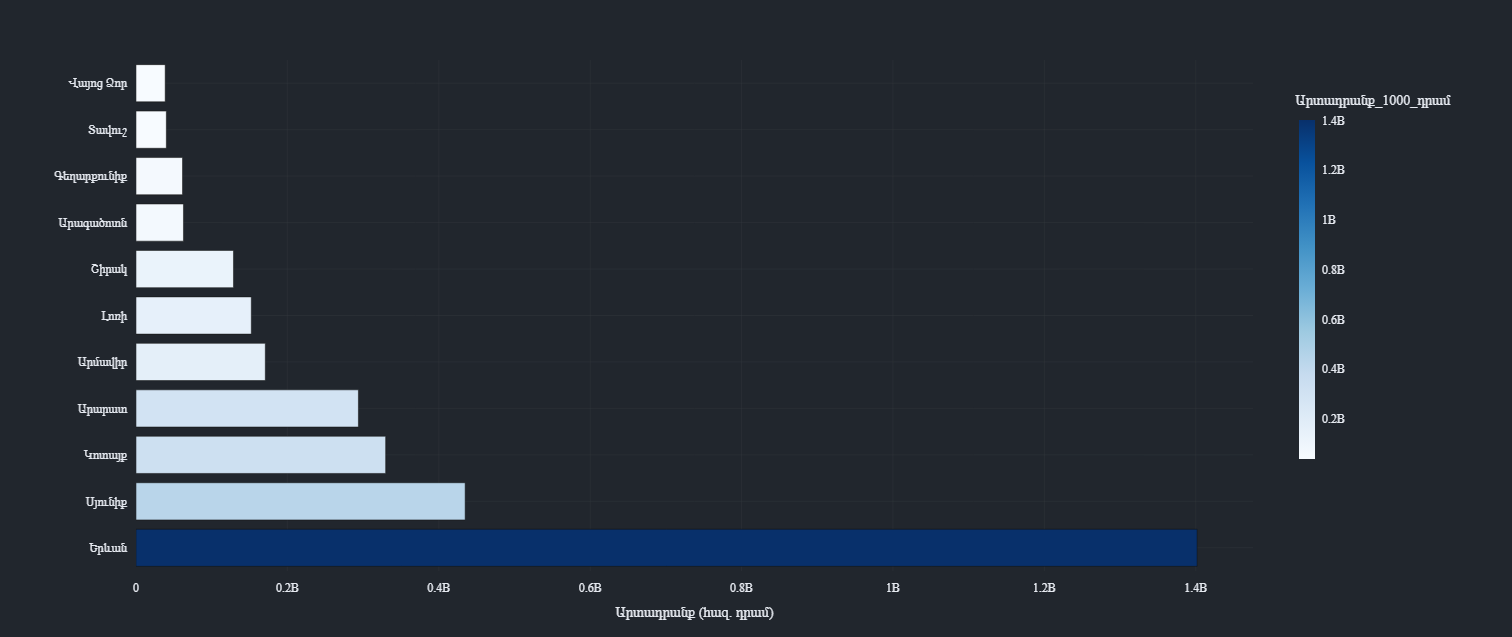
\includegraphics[width=0.8\textwidth]{figures/38_regional_industrial_output.png}
    \caption{Industrial Output by Administrative Region (Marz)}
    \label{fig:regional_industry}
\end{figure}

\begin{figure}[H]
    \centering
    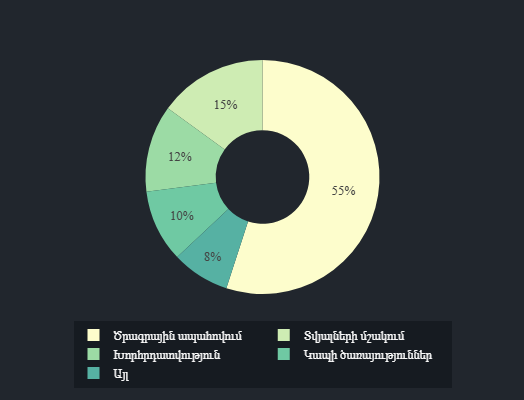
\includegraphics[width=0.8\textwidth]{figures/39_it_sector_structure.png}
    \caption{Internal Composition of the Armenian IT Sector}
    \label{fig:it_structure}
\end{figure}

These figures broaden the analysis beyond aggregate stability. Figure \ref{fig:external_trade} indicates whether domestic growth is accompanied by external rebalancing or by continued import dependence. Figure \ref{fig:utilities} offers a proxy for underlying productive activity. Figure \ref{fig:regional_industry} helps assess whether industrial gains are geographically concentrated. Finally, Figure \ref{fig:it_structure} is essential for evaluating whether Armenia's celebrated IT expansion is broad enough to count as structural transformation. Taken together, these charts suggest that Armenia has made progress toward a more modern economic base, but regional and sectoral concentration remain prominent.\cite{armstatbank,wbTrade2024,wbCPF2025}

\chapter{Integrated Discussion: What Really Drove the Armenian Economy?}
The evidence assembled in this thesis points to a clear but nuanced conclusion. Armenia's economy in 2024--2025 was resilient, yet the resilience was unevenly distributed across sectors and channels. Growth was supported by a favorable combination of external prices, service exports, labor-market tightening, and strong domestic demand. However, not all of these supports are equally durable.

Construction was the largest near-term engine of expansion. It stimulated output, employment, income, and related credit demand. At the same time, it increased Armenia's exposure to property-cycle risk, budget dependence, and banking concentration. This means that the same sector that improved the nowcast also raised the medium-term risk profile of the economy.

The ICT sector represented the strongest candidate for genuine structural upgrading. Its importance lies not only in turnover or employment, but in its potential to support higher productivity, service exports, and wage growth. Yet the labor-market figures suggest that this transformation is constrained by skills and concentration. A modern sector can be strategically important without yet being broad enough to transform the whole economy.

External conditions remained favorable enough to support stability. Commodity prices, remittances, tourism flows, and exchange-rate conditions all contributed to resilience. But these channels are partly exogenous. They can strengthen growth without proving that the domestic economy has become fundamentally less vulnerable.

Inflation remained relatively subdued, which is a positive result. Still, low inflation coexisting with rapid construction, rising wages in selected sectors, and expanding public expenditure should be interpreted as a sign of mixed macro conditions rather than an all-clear signal. In other words, Armenia did not appear to be in generalized overheating, but it did exhibit pockets of sectoral and financial concentration that deserve policy attention.

The central analytical judgment of the thesis is therefore as follows: Armenia's economy was not weak, nor was it simply reverting to pre-shock fragility. It was transitioning from shock-driven expansion toward a more institutionalized growth model, but that model remained incomplete. The positive side of the transition was diversification in services, formal employment, and parts of the external sector. The negative side was a persistent dependence on construction-centered demand and concentrated sources of momentum.

\chapter{Limitations and Directions for Further Research}
This thesis improves substantially on a descriptive dashboard summary, but several limitations remain. First, the analysis relies on a high-frequency monitoring framework rather than a fully estimated structural or dynamic-factor model. Second, some figures combine observed and partial-year data, which limits strict comparability. Third, several important variables for Armenia, including household balance-sheet stress, informal employment quality, and firm-level productivity, are not directly observable in the dashboard. Fourth, the Armenian economy remains exposed to geopolitical shocks that cannot be inferred from historical co-movement alone.

Future research can deepen the contribution in three ways. First, the dashboard can be extended into a formal mixed-frequency nowcasting model with out-of-sample forecast evaluation. Second, more explicit regional analysis could be added to test whether growth dispersion across marzes is narrowing or widening. Third, a more detailed study of construction, real-estate finance, and household affordability would help clarify whether current expansion is sustainable or increasingly speculative.

\chapter{Conclusion}
This thesis set out to evaluate the drivers of Armenian economic performance using a custom high-frequency dashboard and an integrated macroeconomic framework. The evidence indicates that Armenia entered 2025 with meaningful resilience, supported by favorable external conditions, durable service-sector activity, formalizing labor-market trends, and contained inflation. At the same time, the composition of growth was uneven. Construction played an outsized role, financial exposure was concentrated, and much of the economy's apparent strength depended on channels that may not remain equally supportive over time.\cite{imfCR24348,wbPulse2025,cbaImpl2025}

The main conclusion is that Armenia's economy was better understood as \textit{strong but imbalanced} than as simply booming or simply normalizing. The dashboard is useful precisely because it reveals this distinction earlier than annual GDP statistics alone. A credible policy interpretation of the Armenian economy must therefore combine optimism about structural progress, especially in ICT and formal employment, with caution about concentration in construction, public spending dependence, and macro-financial spillovers.

In that sense, the Armenian economy during the period covered by this thesis was not merely growing; it was being restructured in real time. The quality of that restructuring, rather than the headline growth rate alone, is the key issue for future research and policy.

\chapter*{References}
\addcontentsline{toc}{chapter}{References}
\begin{thebibliography}{99}
\bibitem{adbADO2024}
Asian Development Bank.
\textit{Asian Development Outlook, April 2024}.
Available at: \url{https://www.adb.org/sites/default/files/publication/957856/asian-development-outlook-april-2024.pdf}

\bibitem{armstatbank}
Statistical Committee of the Republic of Armenia.
\textit{ArmStatBank}.
Available at: \url{https://statbank.armstat.am/pxweb/en/ArmStatBank/}

\bibitem{cbaMPR2025Q1}
Central Bank of Armenia.
\textit{Monetary Policy Outlook 2025 Q1}.
March 2025.
Available at: \url{https://www.cba.am/Storage/AM/downloads/parberakan/DVQ/Monetary_Policy_Outlook_2025Q1_eng.pdf}

\bibitem{cbaImpl2025}
Central Bank of Armenia.
\textit{Monetary Policy Program Implementation Report (Q2 2024--Q1 2025)}.
May 2025.
Available at: \url{https://www.cba.am/en/reports/8463}

\bibitem{imfCR24348}
International Monetary Fund.
\textit{Republic of Armenia: Fourth Review Under the Stand-By Arrangement and Request for Modifications of Performance Criterion and Monetary Policy Consultation Clause}.
IMF Country Report No. 24/348, December 2024.
Available at: \url{https://www.imf.org/en/Publications/CR/Issues/2024/12/17/Republic-of-Armenia-Fourth-Review-Under-the-Stand-By-Arrangement-and-Request-for-559673}

\bibitem{minfinBudget}
Ministry of Finance of the Republic of Armenia.
\textit{State Budget}.
Available at: \url{https://www.minfin.am/en/page/budget/}

\bibitem{wbCPF2025}
World Bank.
\textit{World Bank Group to Support Job Creation and Resilience in Armenia}.
January 21, 2025.
Available at: \url{https://www.worldbank.org/en/news/press-release/2025/01/21/world-bank-group-to-support-job-creation-and-resilience-in-armenia}

\bibitem{wbMEU2024}
World Bank.
\textit{Armenia Monthly Economic Update -- January 2024}.
Available at: \url{https://thedocs.worldbank.org/en/doc/6b97e748ad629581293fc77a1a9030d5-0080012024/original/ARM-MEU-JAN-2024-Eng.pdf}

\bibitem{wbMEU2025}
World Bank.
\textit{Armenia Monthly Economic Update -- February 2025}.
Available at: \url{https://thedocs.worldbank.org/en/doc/31d4fb42e3f938e12830d2f6339c17fa-0080062025/original/ARM-MEU-FEB-2025-en.pdf}

\bibitem{wbPER2023}
World Bank.
\textit{A New Report by the World Bank Offers a Roadmap for Improving Public Spending Efficiency in Armenia}.
November 9, 2023.
Available at: \url{https://www.worldbank.org/en/news/press-release/2023/11/09/a-new-report-by-the-world-bank-offers-a-roadmap-for-improving-public-spending-efficiency-in-armenia}

\bibitem{wbPulse2025}
World Bank.
\textit{Armenia's Economic Pulse: Fairer Markets for Inclusive Growth}.
Available at: \url{https://www.worldbank.org/en/country/armenia/publication/armenia-economic-pulse-fairer-markets-for-inclusive-growth}

\bibitem{wbTourism2025}
World Bank.
\textit{Armenia to Create Jobs, Attract Private Investment through Stronger Local Tourism Infrastructure}.
April 17, 2025.
Available at: \url{https://www.worldbank.org/en/news/press-release/2025/04/17/armenia-to-create-jobs-attract-private-investment-through-stronger-local-tourism-infrastructure}

\bibitem{wbTrade2024}
World Bank.
\textit{Armenia Trade Competitiveness Diagnostic}.
November 7, 2024.
Available at: \url{https://www.worldbank.org/en/news/factsheet/2024/11/07/armenia-trade-competitiveness-diagnostic}
\end{thebibliography}

\end{document}
